\documentclass[10pt,onecolumn,twoside,a4size]{gsag3jnl}

\articletype{inv} % article type
% {inv} Investigations
% {msr} Mutant Screen Reports
% {gs} Genomic Selection
% {goi} Genetics of Immunity 
% {gos} Genetics of Sex 
% {mp} Multiparental Populations

\usepackage{kotex}
\usepackage{multirow}
\usepackage{subfigure}
\usepackage{mathtools}
\usepackage{mathptmx}
\usepackage{fontspec}
  \setmainfont{BareunBatangL}[BoldFont = BareunBatangB, ItalicFont = Inconsolata-Regular]
  \setsansfont{AppleSDGothicNeo-Regular}[BoldFont = AppleSDGothicNeo-Bold]
  \setmonofont{TimesNewRomanPSMT}[ItalicFont = TimesNewRomanPS-ItalicMT, BoldItalicFont = Times-RomanSC]

\newcommand{\ACL}{AC\textsubscript{L}}
\newcommand{\ACR}{AC\textsubscript{R}}
\newcommand{\PFCL}{PFC\textsubscript{L}}
\newcommand{\PPCL}{PPC\textsubscript{L}}
\newcommand{\iid}{\stackrel{\mathrm{iid}}{\sim}}
\newcommand{\proof}{\texttt{\textit{\textbf{Proof }}}}
\newcommand{\fakesection}[1]{%
  \par\refstepcounter{section}% Increase section counter
  \addcontentsline{toc}{section}{\protect#1}% Add section to ToC
  % Add more content here, if needed.
}

\DeclareMathOperator*{\argmax}{argmax}
\DeclareMathOperator*{\argmin}{argmin}

\linespread{1.5}
\graphicspath{{./Figure/}}
\title{일반화 선형혼합모형(GLMM)을 이용한 청성안정유발반응(ASSR) 연구}

\author[1]{박상현}
\author[$\ast$,1]{장원철}

\affil[]{대한민국 서울특별시 08826, 서울대학교 자연과학대학 통계학과}
\affil[$\ast$]{지도교수}

\keywords{GLMM \\ ASSR \\ Prediction model}

\runningtitle{일반화 선형혼합모형(GLMM)을 이용한 청성안정유발반응(ASSR) 연구} % For use in the footer 

%% For the footnote.
%% Give the last name of the first author if only one author;
% \runningauthor{FirstAuthorLastname}
%% last names of both authors if there are two authors;
% \runningauthor{FirstAuthorLastname and SecondAuthorLastname}
%% last name of the first author followed by et al, if more than two authors.
\runningauthor{박상현, 장원철}

\begin{abstract}
본 연구에서는 청성안정유발반응(auditory steady state evoked responses; ASSR)을 통해 측정된 뇌전도로 행동을 예측하는 모형을 통해 청각 피질(auditory cortex; AC), 전두엽 피질(prefrontal cortex; PFC) 및 두정엽 피질(posterior parietal cortex; PPC)의 뇌전도가 생쥐의 행동 결정에 어떤 방식으로 연관되는지를 밝히려고 시도하였다. 이를 위해 기존 예측 모형의 한계를 지적하고 개선된 예측 모형인 일반화 선형혼합모형(generalized mixed effect model; GLMM)을 제안한다. GLMM은 고정효과(fixed effect)와 랜덤효과(random effect)를 모두 고려함으로써 반복측정으로 인한 상관관계 구조를 반영할 수 있고, 결과적으로 약 .925의 F score를 보였다.
\end{abstract}

\begin{document}

\maketitle
\thispagestyle{firststyle}
\logomark
%\articletypemark
\marginmark
\firstpagefootnote

\correspondingauthoraffiliation{1}{교신저자: 박상현, 대한민국 서울특별시 08826, 서울대학교 자연과학대학 통계학과, Email: lkd1962@naver.com}
\vspace{-34pt}% Only used for adjusting extra space in the left column of the first pages

\setcounter{tocdepth}{2}
\sffamily
\tableofcontents

\normalfont
\section{서론}
\texttt{ASSR}(\texttt{Auditory Steady State Evoked Responses}; 청성안정유발반응) 실험은 주기적으로 빠르게 반복되는 청각 자극에 대한 \texttt{EEG}(\texttt{Electroencephalography})나 \texttt{LFP}(\texttt{Local Field Potential})를 관측하는 실험이다 \texttt{\citep{bohorquez2008generation}}. 1981년 \texttt{Galambos}와 동료들이 40\texttt{Hz}대의 청각 자극에서 안정파 유발반응(\texttt{steady state evoked potential})을 보고한 것을 시작으로 \texttt{\citep{galambos198140}}, \texttt{Rickards, Piocton, Choen} 등이 다양한 주파수에서의 \texttt{ASSR} 반응을 광범위하게 연구하며 신경과학 및 청각 임상에서의 표준적인 실험절차로 자리잡게 되었다 \texttt{\citep{rickards1982steady, picton1987potentials, kuwada1986scalp, cohen1991comparison}}. 특히 이는 다른 자극과는 달리 주어진 주파수에 해당하는 와우(\texttt{cochlea})의 좁은 부위를 자극하여 주파수 특이성이 높고 \texttt{\citep{john2000master}}, 반응의 자동탐지 알고리즘이 잘 개발되어 객관적인 반응 탐지가 가능하다는 장점이 있다 \texttt{\citep{cone2002auditory}}.
 
본 연구에서는 독립성 가정이 위배된다는 점을 해결할 수 있는 방안으로 \texttt{GLMM}(\texttt{Generalized Linear Mixed Effect Model}; 일반화 선형혼합모형)을 이용한 예측을 제안하고자 한다. \texttt{GLMM}은 오차항이 하나인 $t$ 검정이나 \texttt{Wilcoxon} 부호순위합 검정의 모형과는 달리 여러 개의 오차항을 동시에 고려할 수 있는 일반적인 통계 모형으로 반복측정으로 인해 생기는 종속성을 서로 독립으로 간주할 수 있는 여러 개의 오차 원인으로 분해하여 모형에 반영한다 \texttt{\citep{pinheiro2006mixed, agresti2000random}}. 나아가, \texttt{GLMM}은 예측 모형으로도 활용될 수 있다는 장점을 가진다. 물론 예측만을 위한 \texttt{ANN}(\texttt{Artificial Neural Network}) 등의 비모수적 방법이 계산 신경과학 분야에서 널리 이용되고 있지만, 이가 가지는 본질적인 해석의 어려움 때문에 통계적 추론이 필요한 분야에까지 적용되기는 쉽지 않다. \texttt{GLMM}은 모수적인 모형으로서 해석의 용이함을 유지하면서 예측 모형으로도 나쁘지 않은 성능을 발휘한다.

\section{모형 적합}
\subsection{GLMM 모형}
다중선형회귀모형은 설계행렬 $X$, 반응변수 벡터 $\mathbf{Y}$, 회귀계수 벡터 $\beta$, 오차 $\epsilon\sim\mathbf{N}_n(\mathbf{0},\,\sigma^2I_n)$에 대해 다음과 같은 모형으로 정의된다.
\begin{equation*}
  \underset{n\times1}{\mathbf{Y}}=\underset{n\times p}{X}\underset{p\times1}{\beta}+\underset{n\times1}{\epsilon}
\end{equation*}
여기서 $\beta$는 비록 알 수는 없지만 고정된 상수로서, 위의 모형은 설명변수의 가중합에 약간의 오차가 더하여져 반응 $Y$가 결정된다고 보아 이때 가중치의 역할을 하는 $\beta$를 추정하고자 한다. 곧 $Y$의 랜덤성은 오로지 오차 $\epsilon$에 기인한다. 이러한 다중선형회귀모형에 더 이상 상수가 아닌 확률변수를 회귀계수로 추가한 모형을 생각할 수 있는데, 이를 \texttt{LME}(\texttt{Linear Mixed Effect Model}; 선형 혼합모형)라 하며, 다음과 같이 정의된다 \texttt{\citep{demidenko2013mixed}}.
\begin{equation*}
  \underset{n\times1}{\mathbf{Y}}=\underset{n\times p}{X}\underset{p\times1}{\beta}+\underset{n\times q}{Z}\underset{q\times1}{\gamma}+\underset{n\times1}{\epsilon}
\end{equation*}
여기서 $Z$는 랜덤효과 $\gamma$의 설계행렬이며 $\gamma\sim\mathbf{N}_q(\mathbf{0},\,\Psi),\,\epsilon\sim\mathbf{N}_n(\mathbf{0},\,\Sigma)$이고 $\gamma$와 $\epsilon$은 서로 독립으로 가정한다. 새롭게 추가된 랜덤효과 $\gamma$와 구별하기 위해 고정된 상수인 $\beta$를 고정효과라 한다. 랜덤효과의 도입에 더하여 일반적으로 \texttt{LME}에서는 오차항의 분산 또한 더 이상 $\sigma^2I$으로 제한하지 않는다. 따라서 \texttt{LME}에서는 반응 $Y$가 결정되는 데 있어 더 이상 오차 $\epsilon$만이 유일한 랜덤성으로 적용하지 않는다. 설명변수의 가중합에서 가중치의 일부에도 랜덤성이 있다고 보는 것이다. 일견 이렇게 랜덤효과를 도입하는 것이 어떠한 차이를 만드는지 명확하지 않을 수 있으나, 다중선형회귀모형에서 \texttt{indicator variable}을 더미(\texttt{dummy}) 변수로 사용하여 분산분석을 온전히 기술할 수 있듯이 위의 \texttt{LME}는 아주 폭넓은 구조의 자료를 다룰 수 있도록 해 준다 \texttt{\citep{searle2001generalized}}.

이제 \texttt{LME}에서 $\gamma$가 조건부로 주어지면 이때 $\mathbf{Y}\vert\gamma$는 다중선형모형으로 축소된다는 점에 주목하고 다중선형모형을 \texttt{GLM}으로 일반화할 때 사용한 아이디어를 그대로 차용하여 오차가 정규분포가 아닌 경우로 \texttt{LME}를 확장하면 \texttt{GLMM}을 얻는다. 즉, \texttt{overdispersion}이 없는 지수족 분포의 \texttt{PDF}(\texttt{Probability Density Function}; 확률밀도함수) $f(x;\eta)=h(x)\exp(\eta x-A(\eta))$와 적당한 \texttt{link function} $g:\mathbb{R}\to\mathbb{R}$에 대해 \texttt{GLMM}은 
\begin{align}\label{eq:glmm_model}
  &f_{Y_i\vert\gamma}(y_i\vert\gamma)=h(y_i)\exp(\eta_iy_i-A(\eta_i))\\
  &g(\mathbf{E}(Y_i\vert\gamma))=\eta_i=\mathbf{x}_i'\beta+\mathbf{z}_i'\gamma\nonumber
\end{align}
으로 정의된다. 여기서 $\gamma\sim\mathbf{N}_q(\mathbf{0},\,\Psi)$이고 $i=1,\,\cdots,\,n$이며 $\mathbf{x}_i'$와 $\mathbf{z}_i'$는 각각 \texttt{LME}에서의 고정효과의 설계행렬 $X$와 랜덤효과의 설계행렬 $Z$의 $i$번째 행에 대응된다.

전술한 바와 같이 \texttt{GLMM}은 단순히 랜덤효과를 더한다는 표면적인 의미를 넘어 다양한 구조를 갖는 자료를 다룰 수 있도록 해 주는데, 본 연구의 주제인 반복측정된 자료에 이가 어떻게 적용될 수 있는지 살펴보자. 피실험체에 $m$마리에 대해 각각 $n$번 반복측정하여 생성된 자료의 경우, 각 자료간의 독립성은 보장할 수 없겠지만 이때 측정에 더해지는 오차를 피실험체 수준의 오차와 반복측정 수준의 오차로 분해하면 이러한 오차들 간의 독립성은 보장할 수 있을 것이다. 따라서 다음의 로지스틱 선형혼합모형을 생각할 수 있다.
\begin{align}\label{eq:hierachy_model}
  &Y_{ij}\vert\epsilon_i\iid\mathbf{Bern}(p_{ij})\\
  &g(p_{ij})=\underset{p\times1}{\mathbf{x}_{ij}}'\underset{p\times1}{\beta}+\epsilon_i\nonumber
\end{align}
여기서 $g(x)=\log(x/(1-x))$, $\epsilon_i\iid\mathbf{N}(0,\,\sigma^2)$이고 $i=1,\,\cdots,\,m$는 피실험체를 나타내는 첨자이며 $j=1,\,\cdots,\,n$는 특정 피실험체에서 측정된 순서를 나타내는 첨자이다. 위의 모형에서 반복측정 수준의 모형만 보면 $Y_{ij}$는 $i$번째 피실험체의 $j$번째 반복에서의 반응, $p_{ij}$는 설명변수의 선형결합으로 표현되는 모수(베르누이 분포에서의 성공확률)로 이는 고전적인 로지스틱 회귀모형이다. 그러나 위의 모형은 모수 $p_{ij}$에 피실험체 수준의 오차 $\epsilon_i$를 더하여 $Y_{ij}$가 서로 독립이 아니라는 문제점을 해결한다. 즉, 실험 과정에 있어 오차가 매번의 반복에서 발생할 뿐만 아니라, 피실험체를 선택하는 과정에서도 발생하여 더해진다는 것이다. 이때 작용하는 반복측정 수준의 오차와 피실험체 수준의 오차에 대해서는 어느정도 그 독립성을 보장할 수 있기에 이는 신경과학계의 반복측정 실험에 적합한 모형이라 할 수 있다.

이제 $\mathbf{Bern}(p)$의 확률밀도함수가 $h(x)=\mathbf{1}_{\{0,\,1\}}(x),\,\eta=\log(p/(1-p)),\,A(\eta)=-\log(1-p)$에 대해 (여기서 $\mathbf{1}$는 지시함수)
\begin{equation}
  f(x)=h(x)\exp(\eta x-A(\eta))
\end{equation}
와 같이 지수족 분포로 표현될 수 있다는 점을 떠올리면
\begin{equation}
  \underset{mn\times p}{X}=\begin{bmatrix*}
    \mathbf{x}_{11}'\\
    \mathbf{x}_{12}'\\
    \vdots\\
    \mathbf{x}_{mn}'
  \end{bmatrix*},\,\underset{mn\times m}{Z}=\begin{bmatrix*}
    \mathbf{1}_n&\mathbf{0}_n&\cdots&\mathbf{0}_n\\
    \mathbf{0}_n&\mathbf{1}_n&\cdots&\mathbf{0}_n\\
    \vdots&\vdots&\ddots&\vdots\\
    \mathbf{0}_n&\mathbf{0}_n&\cdots&\mathbf{1}_n
  \end{bmatrix*},\,\underset{m\times1}{\gamma}=\begin{bmatrix*}
    \epsilon_1\\
    \epsilon_2\\
    \vdots\\
    \epsilon_m
  \end{bmatrix*}
\end{equation}
와 $\Psi=\sigma^2I_m$, \texttt{logistic link} $g(x)=\log(x/(1-x))$에 대해
\begin{align}
  &f_{Y_{ij}\vert\gamma}(y_{ij}\vert\gamma)=h(y_{ij})\exp(\eta_{ij}y_{ij}-A(\eta_{ij}))\\
  &g(\mathbf{E}(Y_{ij}\vert\gamma))=\eta_{ij}=\mathbf{x}_{ij}'\beta+\mathbf{z}_{ij}'\gamma\nonumber
\end{align}
로 쓸 수 있으며 이때 $\gamma\sim\mathbf{N}_{m}(\mathbf{0},\,\Psi)$가 되어 방금 살펴보았던 \texttt{GLMM}이 된다. (여기서 $\mathbf{z}_{ij}'$는 행렬 $Z$의 $n(i-1)+j$번째 행을 의미한다.) 이로부터 \texttt{GLMM}이 반복측정이 빈번한 신경과학계의 자료에 적합한 모형임을 알 수 있다.

이제 \texttt{GLMM}의 모수 추정과 검정에 대해 생각해보자. \texttt{GLMM} 모형(식 \ref{eq:glmm_model})에서 추정해야 할 모수로는 고정효과 $\beta$와 분산구조 $\Psi$가 있다. 여기서 $\gamma$는 랜덤효과로 고정된 미지의 상수가 아니므로 추정의 대상이 아니다. \texttt{GLM}에서와 마찬가지로 추정은 \texttt{MLE}(\texttt{Maximum Likelihood Estimation}; 최대가능도추정)을 이용하는데, $\mathbf{Y}$의 로그가능도함수를 구하면 분산구조 $\Psi$를 알고 있다는 가정 하에 베이즈 정리로부터 다음과 같이 구해진다.
\begin{align}
  l(\beta)&=\log\int_{\mathbb{R}^q}f_{\mathbf{Y}\vert\gamma}(\mathbf{Y}\vert\gamma)f_\gamma(\gamma)\,d\gamma\\
  &=\log\int_{\mathbb{R}^q}\exp\bigg(\sum_{i=1}^n[\mathbf{z}_i'\gamma Y_i-A(\mathbf{x}_i'\beta+\mathbf{z}_i'\gamma)]-\frac{\gamma'\Psi^{-1}\gamma}{2}\bigg)\,d\gamma-\frac{1}{2}\log\det\Psi+\sum_{i=1}^n\mathbf{x}_i'\beta Y_i+\mathrm{const.}\nonumber
\end{align}
대부분의 경우 위 식의 적분이 닫힌 형태로 구해지지 않으므로 \texttt{adaptive GHQ}(\texttt{Gauss-Hermite Quadrature})나 라플라스 근사, \texttt{MCMC}(\texttt{Markov Chain Monte Carlo Simulation}), \texttt{MCEM}(\texttt{Monte Carlo Expectation Maximization}) 등을 통한 수치적분 기법으로 적분을 근사하여 계산한다 \texttt{\citep{capanu2013assessment}}. 실제로는 대부분의 경우 분산구조 $\Psi$ 또한 알지 못하므로 이를 동시에 추정해야 하고, 이를 위해 적당한 초기값에서 시작하여 조금씩 $\Psi$와 $\beta$를 \texttt{update}하는 반복 알고리즘이 사용된다.

\texttt{GLMM}을 적합한 이후에는 특정 고정효과 $\beta_i$ 대해 가설 $H_0:\beta_i=0$을 검정하거나 특정 랜덤효과 $\gamma$에 대응되는 분산 $\sigma_\gamma^2$에 대해 가설 $H_0:\sigma^2_\gamma=0$을 검정함으로써 관심 있는 뇌 활동이 반응의 유무에 유의미한 영향을 주는지에 대한 통계적 추론을 진행할 수 있다. 먼저 고정효과 $\beta$에 대해 보다 일반적인 선형가설 $H_0:T\beta=\xi\in\mathbb{R}^r$ (단, $\mathrm{rk}\,T=r<p$)을 검정하는 경우, 이를 검정하는 방법으로 크게 \texttt{LRT}(\texttt{Likelihood Ratio test}; 가능도비 검정), \texttt{Wald} 검정, \texttt{Rao} 검정을 생각해볼 수 있다. 각 검정은 다음 검정통계량의 계산을 필요로 한다.
\begin{align}
  \Lambda&=-2[l(\widehat{\beta},\,\widehat{\psi})-l(\widetilde{\beta},\,\widetilde{\psi})]\\
  W&=(T\widehat{\beta}-\xi)'\{T[\nabla^2_\beta l(\widehat{\beta},\,\widehat{\Psi})]^{-1}T'\}^{-1}(T\widehat{\beta}-\xi)\\
  R&=\nabla_\beta l(\widetilde{\beta},\,\widetilde{\Psi})'[\nabla^2_\beta l(\widetilde{\beta},\,\widetilde{\Psi})]^{-1}\nabla_\beta l\widetilde{\beta},\,\widetilde{\Psi})
\end{align}
여기서 $\widehat{\beta}$와 $\widehat{\Psi}$는 각각 \texttt{full model}의 $\beta$와 $\Psi$의 \texttt{MLE}이며 $\widetilde{\beta}$와 $\widetilde{\Psi}$는 각각 귀무가설 하에서 \texttt{reduced model}의 $\beta$와 $\Psi$의 \texttt{MLE}이다. 그렇다면 $\Lambda,\,W,\,R\Rightarrow\chi^2(p-r)$임을 보일 수 있고, 이로부터 신뢰수준 $\alpha$의 (근사적인) 기각역을 정할 수 있다. 각 검정에는 나름의 장단점이 있는데, \texttt{LRT}의 경우 \texttt{full model}에서의 \texttt{MLE}와 \texttt{reduced model}에서의 \texttt{MLE}를 모두 계산하여야 하므로 비교적 많은 계산을 필요로 하지만 다른 두 검정에 비해 정확하며, \texttt{Wald} 검정과 \texttt{Rao} 검정의 경우 \texttt{full model}에서의 \texttt{MLE}와 \texttt{reduced model}에서의 \texttt{MLE} 중 하나만 계산하면 되지만 그 검정통계량 자체가 \texttt{LRT}의 근사이므로 비교적 덜 정확하다. 다만, 근사적으로 세 검정은 모두 동치임이 알려져 있다 \texttt{\citep{tuerlinckx2006statistical}}. 이와 비슷하게 랜덤효과의 분산 성분에 대하여서도 \texttt{LRT}를 수행할 수 있지만, 검정통계량의 극한분포가 카이제곱분포가 아니므로 특별한 경우가 아닌 이상 \texttt{MCMC}와 같은 시뮬레이션 기법을 통해 그 분포를 수치적으로 근사해야 하는 어려움이 있다 \texttt{\citep{zhang2008variance}}.

랜덤효과 $\gamma$의 경우, 전술하였다시피 이는 추정의 대상이 아니다. 대신 그 \texttt{realization}에 대한 예측은 가능한데, 관측값 $\mathbf{Y}$가 주어지고 고정효과 $\beta$와 분산구조 $\Psi$를 알고 있다면 랜덤효과에 대한 예측값으로 \texttt{MSPE}(\texttt{Mean Squared Prediction Error})를 최소화하는 조건부기댓값을 생각해볼 수 있다.
\begin{equation}
  \widetilde{\gamma}=\mathbf{E}_{\beta,\,\Psi}(\gamma\vert\mathbf{Y})=\argmin_{\gamma_*\in\mathbb{R}^q}\mathbf{E}_{\beta,\,\Psi}||\gamma-\gamma_*||^2
\end{equation}
실제로는 $\beta$와 $\Psi$를 알지 못하므로 이를 앞서 소개한 방법들을 이용하여 구한 추정량 $\widehat{\beta}$와 $\widehat{\Psi}$으로 대신하여 $\gamma$를 다음과 같이 예측할 수 있다 \texttt{\citep{mcculloch2011prediction}}.
\begin{align}
  \widetilde{\gamma}&=\mathbf{E}_{\widehat{\beta},\,\widehat{\Psi}}(\gamma\vert\mathbf{Y})=\frac{\int_{\mathbb{R}^q}\gamma f_{\mathbf{Y}\vert\gamma}(\mathbf{Y}\vert\gamma)f_\gamma(\gamma)\,d\gamma}{\int_{\mathbb{R}^q}f_{\mathbf{Y}\vert\gamma}(\mathbf{Y}\vert\gamma)f_\gamma(\gamma)\,d\gamma}\\
  &=\frac{\int_{\mathbb{R}^q}\gamma\exp(\sum_{i=1}^n[\mathbf{z}_i'\gamma y_i-A(\mathbf{x}_i'\widehat{\beta} y_i+\mathbf{z}_i'\gamma y_i)]-\gamma'\widehat{\Psi}^{-1}\gamma/2)\,d\gamma}{\int_{\mathbb{R}^q}\exp(\sum_{i=1}^n[\mathbf{z}_i'\gamma y_i-A(\mathbf{x}_i'\widehat{\beta} y_i+\mathbf{z}_i'\gamma y_i)]-\gamma'\widehat{\Psi}^{-1}\gamma/2)\,d\gamma}\nonumber
\end{align}
이를 본 연구에서 사용할 모형(식 \ref{eq:hierachy_model})에 적용하면 $i$번째 피실험체의 새로운 뇌 활동 정보 $\mathbf{x}_*\in\mathbb{R}^p$에 대해 반응 유무의 확률 $p_*\in[0,\,1]$를 다음과 같이 예측할 수 있다.
\begin{equation}
  \widetilde{p}_*=g^{-1}(\mathbf{x}_*'\widehat{\beta}+\widetilde{\epsilon}_i)
\end{equation}
곧, \texttt{GLMM}은 반응 유무를 예측하는 예측모형으로도 활용할 수 있어 해석의 용이함과 활용성을 두루 갖춘 모형이다.

\subsection{자료 전처리}
\paragraph{이상 채널 제거}

전기적인 신호로 측정되는 뇌파에는 뇌의 활동 이외에도 각종 잡음이 뒤섞이어 기록된다. 일반적으로 이러한 잡음을 뇌파에서 분리해 내는 것은 쉬운 일이 아니며, 이에 대한 다양한 시도와 제안이 이루어져 왔다 \texttt{\citep{shoker2005artifact, nolan2010faster,lawhern2013detect, mognon2011adjust}}. 하지만 이들은 대부분 사람의 두피에서 측정된 \texttt{EEG}에서의 잡음 제거를 목적으로 고안된 방법들이어서 본 실험에서 사용된 쥐의 \texttt{LFP}에 곧바로 적용하기에는 어려움이 있다. 또한, 사람의 \texttt{EEG}에서의 잡음의 주된 요인이 피험자의 눈깜빡임과 같은 필수불가결한 생리적 활동이나 두피에서의 전기 신호의 간섭에 기인하는 반면, 쥐의 \texttt{LFP}에서는 이러한 요인들로 인한 잡음이 거의 없어 비교적 잡음이 영향이 적다.  그럼에도 불구하고 측정 전극 자체의 이상과 같은 이유로 극히 비정상적인 \texttt{LFP}가 기록되는 경우가 있는데, 다행히 이런 경우는 그림 \ref{fig:LFP_raw}과 같이 \texttt{LFP}의 시계열도를 직접 그려봄으로써 육안으로 그 이상유무를 쉽게 판단할 수 있다. 본 연구에서는 보수적인 방식을 택하여 이상이 있는 채널의 자료를 제거하고 분석을 수행하였다. 이상이 있는 것으로 판단된 채널은 표 \ref{tab:bad_chan}과 같다.

\begin{table}[tp]
  \linespread{1}
  \renewcommand{\familydefault}{\sfdefault}\normalfont
  \centering
  \caption{\bf 이상이 있는 것으로 판단되어 분석에서 제외된 채널}
  \begin{tabularx}{\linewidth}{cXXXXXXXX}
  \hline
  \header 피실험체 & 1 & 2 & 3 & 4 & 5 & 6 & 7 & 8\\
  \hline
  이상채널 & \ACL & \PFCL & BF & BF & BF & - & \ACL, BF & -\\
  \hline
  \end{tabularx}
  \label{tab:bad_chan}
\end{table}

\begin{figure}[tp]
  \renewcommand{\familydefault}{\sfdefault}\normalfont
  \centering
  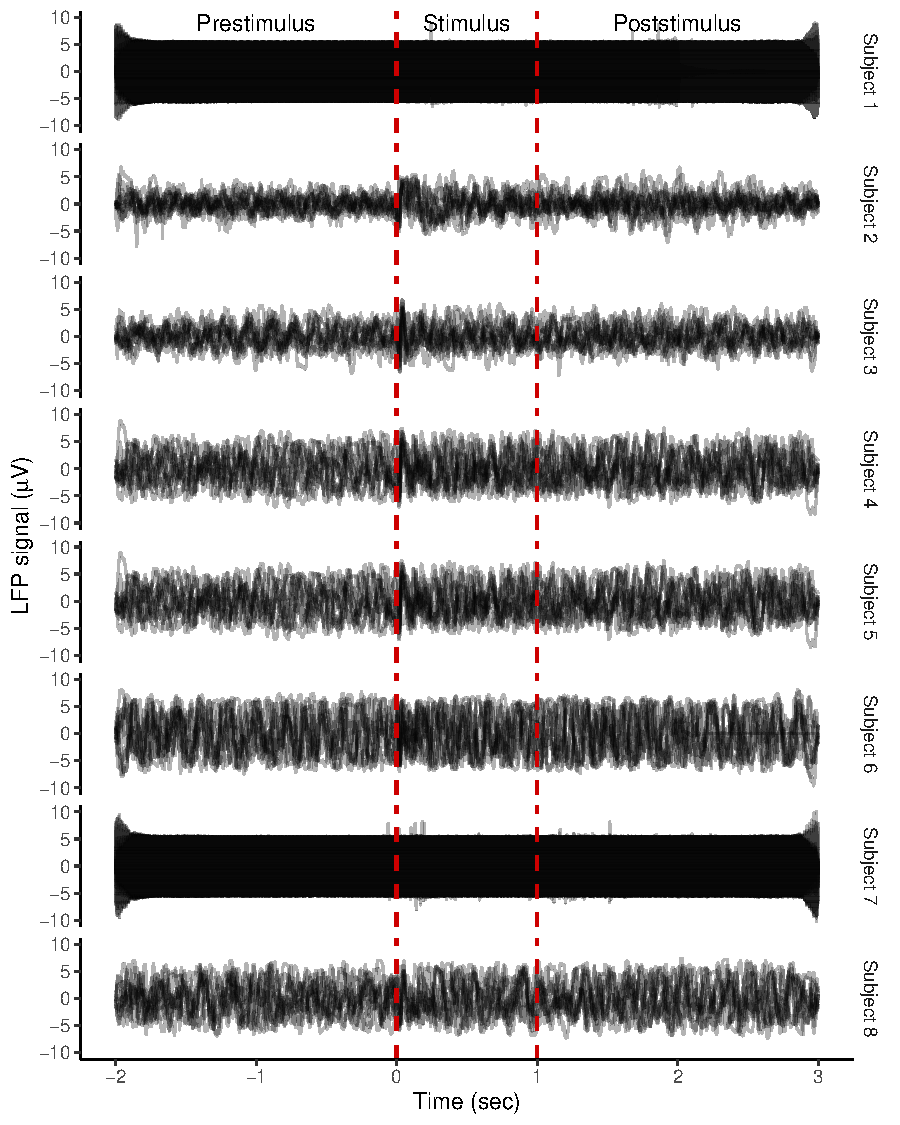
\includegraphics[width=0.7\linewidth]{LFP_raw.pdf}
  \caption{\small \ACL 채널에서 측정된 LFP의 시계열도. 각 피실험체 별로 자극이 시작된 순간을 0초로 하여 세션 1의 첫 10번의 시행에서 관측한 자료를 겹쳐서 나타내었다. 빨간 점선은 prestimulus, stimulus, poststimulus 구간을 나타낸다. 육안으로도 쉽게 1번과 7번 피실험체의 \ACL 채널 전극에 이상이 있음을 명백히 알 수 있다. 한편, 자극이 시작되는 0초 부근에서 펄스 형태의 뇌파가 지속적으로 관측된다는 점도 확인할 수 있다.}
  \label{fig:LFP_raw}
\end{figure}

\paragraph{LFP 정규화}

여러 피실험체 간의 \texttt{LFP}를 비교하기 위해 이들을 적당히 정규화하는 작업이 필요하다. 우선 총 5초의 \texttt{LFP} 중에서 분석의 대상인 \texttt{prestmulus} 기간인 -2초부터 0초까지의 자료만을 잘라내었다.\footnote{이때, 자료의 양 끝에서 왜곡이 발생하는 것을 막기 위해 실제로는 0.2초의 \texttt{epoch}을 두고 -1.8초부터 -0.2초까지를 잘랐다. 실제로, 그림 \ref{fig:LFP_raw}을 보면 자극이 시작된 0초 부근에서 펄스 형태가 일관되게 관측됨을 알 수 있다. 이러한 뇌파는 청각 자극의 제시에 따른 것으로, 자극이 주어지기 이전의 자료만을 바탕으로 자극에 대한 반응의 상관관계를 분석하는 본 분석의 목표에 비추어 보았을 때 고려되지 않아아 함이 타당하다.} 다음으로, 한 시행에서 관측한 \texttt{LFP}의 표본평균이 0이 되도록 조정해 주었다. 이 이상의 정규화는 이후 분석에 영향을 줄 수 있다고 판단하여 진행하지 않았다.

\paragraph{Bandpower 계산}

\texttt{LFP}를 시계열로 생각하여 이를 그대로 분석하는 것도 하나의 방법이겠으나, 신경과학계에서는 \texttt{LFP}의 \texttt{bandpower}를 분석하는 경우가 많다. 이는 특정 주파수대의 \texttt{bandpower}가 나름의 의미를 가지는 것으로 밝혀져 있어 이후 분석 결과의 해석이 용이하기 때문이다 \texttt{\citep{subha2010eeg}}. 이러한 관례를 따라 본 연구에서도 \texttt{LFP}의 \texttt{bandpower}를 계산하여 사용하였다.

시계열 $\{X_t\}$에 대해 이의 푸리에 변환을 $\{\widetilde{X}_\omega\}$라 하면 $\{X_t\}$의 \texttt{PSD}(\texttt{Power Spectral Density}; 스펙트럼 밀도) $S_X(\omega)$는 다음과 같이 정의된다.
\begin{equation}
  S_X(\omega)=\mathbf{E}|\widetilde{X}_\omega|^2
\end{equation}
하지만, 일반적으로 임의의 시계열에 대해 그 푸리에 변환이 존재함을 보장할 수 없으므로 적분의 순서를 바꾸어 $\{X_t\}$의 \texttt{PSD}를
\begin{equation}
  S_X(\omega)=\lim_{T\to\infty}\mathbf{E}\left|\frac{1}{\sqrt{T}}\int_0^TX_te^{-\mathbf{i}\omega t}\,dt\right|
\end{equation}
로 정의하는 경우가 많다 \texttt{\citep{miller2012probability}}. 여기서 $\mathbf{i}$는 허수단위이다. 이제 주어진 주파수대(\texttt{band}) $I\subseteq\mathbb{R}$에 대해 \texttt{bandpower} $\mathrm{BP}_I$는 $I$에서의 $S_X$의 적분, 즉
\begin{equation}
  \mathrm{BP}_I=\int_IS_X(\omega)\,d\omega
\end{equation}
로 정의된다.

실제로는 모든 $t\in\mathbb{R}$에 대해 $X_t$를 관측하지 못하므로 \texttt{PSD}를 추정해야 한다. 그 방법에는 \texttt{Bartlett}의 방법, \texttt{LSSA}(\texttt{Least Squares Spectral Analysis}) 등과 같은 비모수적인 방법부터 \texttt{ARMA}(\texttt{AutoRegressive Moving Average}) 추정, \texttt{MUSIC}(\texttt{MUltiple SIgnal Classification}) 방법 등 모수적인 방법에 이르기까지 다양한 방법이 제시된 바 있으며 현재도 \texttt{SDE}(\texttt{Spectral Density Estimation})이라는 분야로 활발히 연구되고 있다 \texttt{\citep{stoica2005spectral}}. 여기에서는 비모수적인 방법 중 비교적 단순하면서도 널리 사용되는 방법으로, 관측된 자료를 \texttt{DFT}(\texttt{Discrete Fourier Transform})하여 \texttt{periodogram}을 구한 다음 이를 \texttt{PSD}의 추정량으로 사용하였다. 이후 추정된 \texttt{PSD}의 $I$에서의 적분을 사각형법으로 근사하여 최종적인 \texttt{bandpower}의 추정량을 얻었다.

실제 계산에는 \texttt{MATLAB} 함수 \textit{bandpower}가 사용되었으며 이때 사용한 주파수대 $I$는 표 \ref{tab:band_freq}와 같다. 각각의 주파수대는 전술한 바와 같이 신경과학계에서 이미 광범위하게 연구되어 나름의 의미가 많이 밝혀져 있다 \texttt{\citep{ehlers1997slow, vertes2005hippocampal, baker2007oscillatory, crick1990towards}}.

\begin{table}[tp]
  \linespread{1}
  \renewcommand{\familydefault}{\sfdefault}\normalfont
  \centering
  \caption{\textbf{신경과학계에서 흔히 분석하는 주파수대}}
  \begin{tabularx}{\linewidth}{lXXXXX}
  \hline
  \header 명칭 & {Delta} & {Theta} & {Beta} & {Gamma} & {High gamma}\\
  \hline
  주파수대(Hz) & $[1,\,4]$ & $[4,\,12]$ & $[12,\,30]$ & $[30,\,50]$ & $[50,\,100]$\\
  % 약칭 & $\delta$ & $\theta$ & $\beta$ & $\gamma$ & $\gamma^+$\\
  \hline
  \end{tabularx}
  \label{tab:band_freq}
\end{table}


\subsection{탐색적 자료분석}

\texttt{GLMM} 적합에 앞서, 간단한 탐색적 자료분석을 수행하였다. 먼저, 각 피실험체별로 \texttt{Hit} 그룹과 \texttt{Miss} 그룹의 \texttt{bandpower} 분포를 살펴보았다. 그림 \ref{fig:EDA}의 \texttt{A}, \texttt{C}는 \texttt{\ACL} 채널 \texttt{beta band}의 \texttt{bandpower} 분포를 나타낸 것으로서, 이로부터 \texttt{bandpower}의 분포가 심하게 \texttt{right-skew}되어 있음을 알 수 있다. 이는 다른 채널이나 다른 주파수대에 대해서도 마찬가지였다. 이후 분석의 편의를 위해 \texttt{bandpower}에 로그 변환을 취하였다.

\begin{figure*}[tp]
  \renewcommand{\familydefault}{\sfdefault}\normalfont
  \centering
  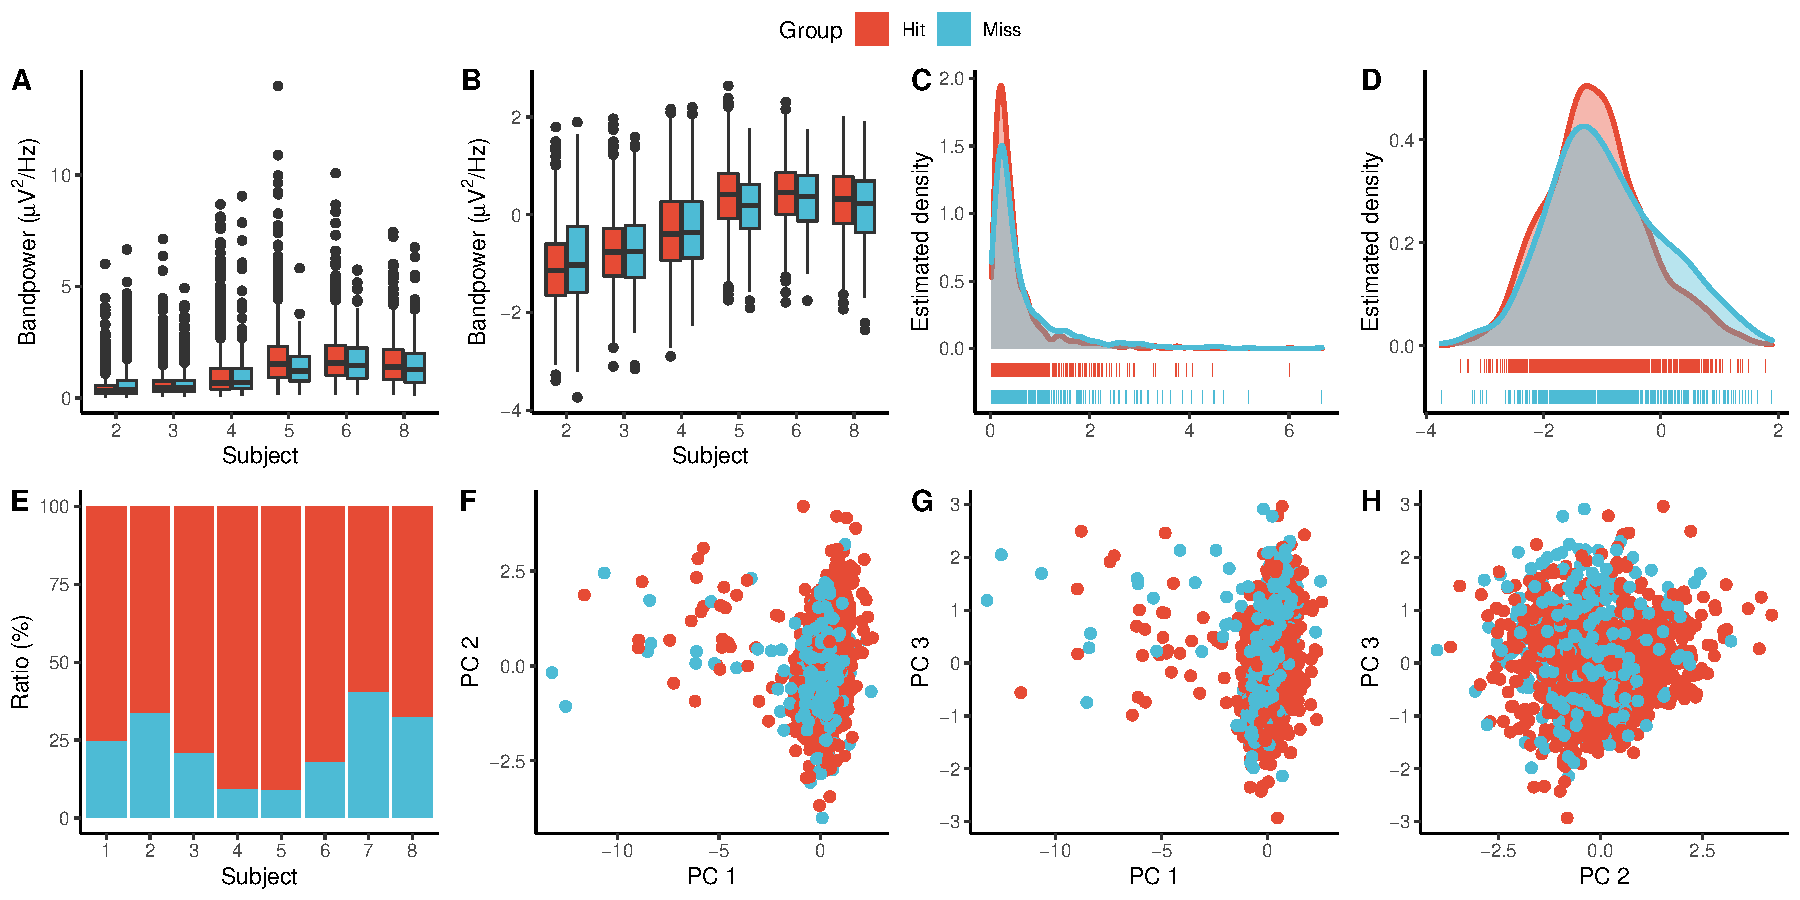
\includegraphics[width=\linewidth]{EDA.pdf}
  \caption{\small 로그 변환 \textbf{A} 전과 \textbf{B} 후 \ACL 채널 delta band의 bandpower로 그린 box plot. 그 중에서 2번 피실험체의 로그 변환 \textbf{C} 전과 \textbf{D} 후의 추정된 분포. 추정된 분포는 Gaussian 커널을 이용한 커널분포추정의 결과이며 이때의 bandwidth는 $0.9n^{-1/5}\min\{\widehat{\sigma},\,\mathrm{IQR}/1.34\}$로 추정하였다 (로그 변환 전 Hit: 0.0609, Miss: 0.1143, 로그 변환 후 Hit: 0.1789, Miss: 0.2590). 여기서 $n$은 표본의 수이며 $\widehat{\sigma}$는 표본표준편차이다. \textbf{E} 피실험체별 {Hit} 그룹과 {Miss} 그룹 간의 비율. 피실험체에 따라 {Hit}의 비율이 {Miss} 비율보다 작게는 1.5배(피실험체 7)에서 많게는 10.4배(피실험체 5) 가량 더 많았다. \textbf{F}$\sim$\textbf{H} 1번 피실험체의 3개의 주성분을 추출하여 그린 산점도. 어느 주성분 방향에서 보나 두 그룹이 서로 거의 구분이 되지 않고 잘 섞여 있음을 알 수 있다. 주성분 분석에는 R 함수 \textrm{\textit{prcomp}}이 사용되었으며 피실험체별로 이상 채널을 제외한 모든 채널에서의 bandpower를 하나의 변량으로 하여 주성분분석을 수행하였다. 이때, 각 변량의 단위가 모두 같은 것을 고려하여 scaling은 하지 않았다.}
  \label{fig:EDA}
\end{figure*}

다음으로, 각 피실험체별로 \texttt{Hit} 그룹과 \texttt{Miss} 그룹 간의 비율을 살펴보았다. 그림 \ref{fig:EDA}의 \texttt{E}는 그 비율을 그래프로 나타낸 것인데, 이로부터 \texttt{Hit} 그룹이 \texttt{Miss} 그룹보다 훨씬 더 많은, 두 그룹간의 불균형이 뚜렷한 자료임을 확인할 수 있다.

이어서 두 그룹이 서로 어떻게 섞여 있는지를 보기 위해 각 피실험체별로 \texttt{PCA}(\texttt{Principal Component Analysis}; 주성분분석)를 수행하였다. 그림 \ref{fig:EDA}의 \texttt{F}$\sim$\texttt{H}는 그 중 1번 피실험체의 3개의 주성분으로 그린 산점도로, \texttt{Hit}과 \texttt{Miss} 두 그룹이 서로 거의 구분이 되지 않고 잘 섞여 있음을 알 수 있다. 다른 피실험체의 경우에도 이와 비슷하였다.

\subsection{GLMM 모형 적합}

모형 기술의 편의를 위해 $i$번째 피실험체의 $j$번째 세션의 $i$번째 시행에서 피실험체가 \texttt{GO} 자극에 튜브를 핥았으면 (\texttt{Hit}이면) $Y_{ijk}=1$ 그렇지 않았으면 (\texttt{Miss} 이면) $Y_{ijk}=0$이라 하자. 또한, 해당 시행에서 \texttt{A} 부위에서 관측된 $I$ 주파수대의 \texttt{bandpower}를 $\mathrm{BP}_{ijk}^I(\mathrm{A})$로 쓰자. 예컨대 해당 시행에서 \texttt{\ACL}의 \texttt{delta} 주파수대에 해당하는 \texttt{bandpower}는 $\mathrm{BP}_{ijk}^\delta(\mathrm{\ACL})$이다. 그렇다면 \texttt{GLMM}에서의 설명변수는 벡터
\begin{equation}
  \underset{25\times1}{\mathbf{x}_{ijk}}=\begin{bmatrix*}
    \mathrm{BP}_{ijk}^\delta(\mathrm{\ACL})\\
    \mathrm{BP}_{ijk}^\theta(\mathrm{\ACL})\\
    \vdots\\
    \mathrm{BP}_{ijk}^{\gamma^+}(\mathrm{\PPCL})\\
  \end{bmatrix*}
\end{equation}
로 쓸 수 있다. 다만, 앞서 데이터 전처리 과정에서 본 바와 같이 피실험체마다 이상 채널이 있으므로 25개의 설명변수를 다 쓰지는 못하고, \texttt{BF} 채널의 자료와 1, 2, 7번 피실험체의 자료를 제외한 차원이 20인 도합 3026개의 자료를 분석하였다.

앞서 \texttt{GLMM}을 소개하며 생각한 모형과는 달리, 이 실험에서는 반복측정이 시행 수준과 세션 수준의 두 가지 단계로 중첩되어 이루어졌다. 따라서 시행 수준, 세션 수준, 피실험체 수준에서 각각 서로 독립인 오차가 발생함을 기술하는 다음과 같은 \texttt{GLMM}을 생각하자.
\begin{align}\label{eq:glmm_example}
  &Y_{ijk}\vert\epsilon_{ij},\,\varphi_i\iid\mathbf{Bern}(p_{ijk})\\
  &g(p_{ijk})=\mathbf{x}_{ijk}'\beta+\epsilon_{ij}+\varphi_i\nonumber
\end{align}
여기서 $g(x)=\log(x/(1-x))$이며 $\epsilon_{ij}\iid\mathbf{N}(0,\,\sigma^2),\,\varphi_i\iid\mathbf{N}(0,\,\tau^2)$고 서로 독립이다. \texttt{GLM}의 적합과정을 비슷하게 따라간다고 한다면, 20개의 설명변수를 모두 사용하여 적합을 한 후에 \texttt{AIC}(\texttt{Akaike information criterion}; \texttt{Akaike} 정보기준)나 \texttt{BIC}(\texttt{Bayesian information criterion}; 베이지안 정보기준)등을 사용하여 모형 선택의 과정을 거쳐야 할 것이다. 충분한 시간과 컴퓨팅 자원이 있다면 이렇게 할 수 있겠지만, 한 번의 적합에 비교적 오랜 시간이 걸리는 \texttt{GLMM}의 특성상 20개나 되는 변수를 모두 사용하여 모형 선택을 진행하는 것은 현실적으로 쉽지 않다. 이에 본 연구에서는 \texttt{elastic net}을 이용하여 설명변수 중 일부를 선별(\texttt{prescreening})하는 방식을 택하였다.

\texttt{Elastic net}은 기존의 \texttt{ridge regression}과 \texttt{LASSO}(\texttt{Least Absolute Shrinkage and Selection Operator})의 아이디어를 합한 것으로, 편차와 분산의 균형을 잡아 평균제곱오차를 줄이는 동시에 모형의 \texttt{sparsity}를 추구하는 것을 목표로 한다. 이를 위해 \texttt{elastic net}은 계수 추정을 위한 목적함수에 $L_1$ 패널티와 $L_2$ 패널티를 추가하여 다음과 같이 계수를 추정한다 \texttt{\citep{friedman2010regularization}}.
\begin{equation}
  \widehat{\beta}=\argmin_{\beta\in\mathbb{R}^p}\bigg\{-l(\beta)+\lambda\bigg[\alpha\frac{||\beta||_2^2}{2}+(1-\alpha)||\beta||_1\bigg]\bigg\}
\end{equation}
여기서 $l$은 모형의 로그가능도이며, $\lambda\geq0,\,\alpha\in[0,\,1]$는 각각 패널티의 정도와 두 패널티간의 균형을 조절하는 \texttt{hyperparameter}로 사용자가 적절히 설정해주어야 하는 값이다.

본 연구에서 최종적으로 적합하고자 하는 모형이 로지스틱 \texttt{GLMM}이므로 로지스틱 \texttt{GLM}에 \texttt{elastic net}을 사용하여 변수 선별을 진행하였다. \texttt{Hyperparameter tuning}은 10-\texttt{fold CV}를 통해 구한 \texttt{AUC}(\texttt{Area Under the Curve})를 기준으로 \texttt{1sd rule}을 적용하였다. \texttt{Tunning} 결과 $\alpha=0.15,\,\lambda=0.0118$가 선택되었으며 해당 $\alpha$와 $\beta$로 \texttt{elastic net}을 적합한 결과 20개의 변수 중 17개의 변수가 선별되었다. 그림 \ref{fig:e_net_tuning}과 표 \ref{tab:e_net_select}는 각각 \texttt{hyperparameter tuning} 결과와 변수 선별 결과를 나타낸 것이다.

\begin{table}[tp]
  \linespread{1}
  \renewcommand{\familydefault}{\sfdefault}\normalfont
  \centering
  \caption{\bf Elatsic net으로 선별된 설명변수}
  \begin{tabularx}{\linewidth}{cX}
  \hline
  \header 채널 & 주파수대\\
  \hline
  \ACL & delta, gamma, high gamma\\
  \ACR & delta, theta, beta, gamma, high gamma\\
  \PFCL & delta, theta, beta, gamma, high gamma\\
  \PPCL & delta, theta, beta, high gamma\\
  \hline
  \end{tabularx}
  \label{tab:e_net_select}
\end{table}

\begin{figure}[tp]
  \renewcommand{\familydefault}{\sfdefault}\normalfont
  \centering
  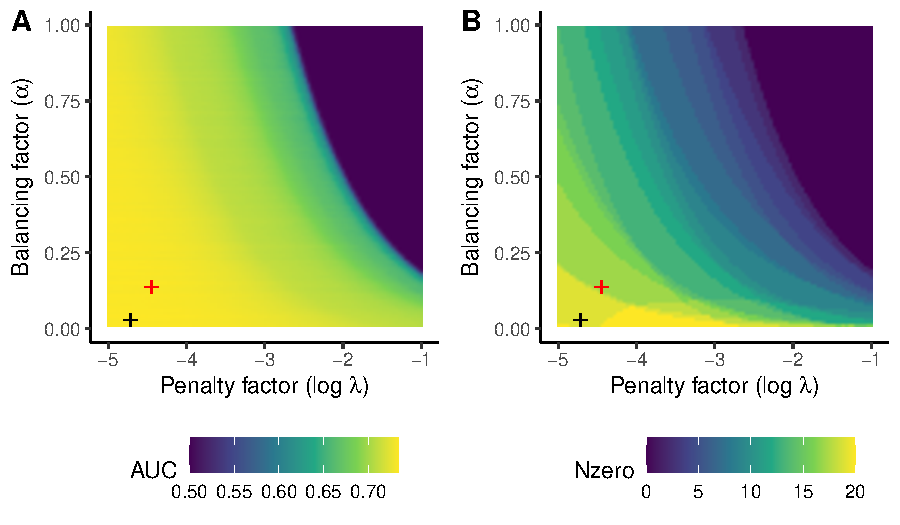
\includegraphics[width=0.7\linewidth]{Enet.pdf}
  \caption{\small Elastic net의 hyperparameter tuning 결과. $\alpha=0.01i$ ($i=1,\,\cdots,\,99$)와 $\lambda=e^{-1-0.04i}$ ($i=0,\,\cdots,\,100$)에 대해 grid search를 수행하였다. 각 조합에 대해 5번의 10-fold CV를 통해 계산된 \textbf{A} AUC와 \textbf{B} 선별된 변수의 수. AUC의 최댓값은 $\alpha=0.04,\,\lambda=0.0089$ ($\mathrm{AUC}=0.7340$, 19개의 변수 모두 사용)에서 얻어졌으며 (검은색 +), 이에 1sd rule을 적용하여 얻은 sparse한 모형은 $\alpha=0.15,\,\lambda=0.0118$ ($\mathrm{AUC}=0.7332$, 17개의 변수 사용)에서 얻어졌다 (빨간색 +). 피실험체를 indicator variable로 하여 elastic net을 적합하였으며 그 적합에는 \texttt{R} 함수 \textrm{\textit{glmnet}}(glmnet 패키지)을 사용하였다.}
  \label{fig:e_net_tuning}
\end{figure}

\subsection{CV 및 시뮬레이션}

전술하였던 바와 같이 \texttt{GLMM}은 예측 모형으로도 활용할 수 있다. 만약 적합한 \texttt{GLMM}이 다른 방법들에 비해 높은 성능을 발휘한다면 이는 \texttt{GLMM}이 \texttt{true model}이라는 강한 증거로 사용될 수 있을 것이고, 더 높은 성능의 예측모형을 개발의 좋은 출발점으로 삼을 수도 있을 것이다. 이러한 \texttt{GLMM}의 장점을 앞서 적합한 \texttt{GLMM}으로써 보이기 위해 주어진 \texttt{bandpower}로부터 피실험체의 반응을 예측하는 다양한 모형을 적합하고, 이를 서로 비교해보았다.

비교의 기준으로 삼을 통계량은 \texttt{AUC}, \texttt{F score}, \texttt{MCC}(\texttt{Matthews correlation coefficient})이며 각각 다음과 같이 정의된다. (여기서는 \texttt{Hit}을 \texttt{True}로 생각한다.)
\begin{align}
  \mathrm{AUC}&=\int\mathrm{ROC}\\
  \texttt{F score}&=\frac{2\mathrm{TP}}{2\mathrm{TP}+\mathrm{FP}+\mathrm{FN}}\nonumber\\
  \mathrm{MCC}&=\frac{\mathrm{TP}\times\mathrm{TN}-\mathrm{FP}\times\mathrm{FN}}{\sqrt{(\mathrm{TP}+\mathrm{FP})(\mathrm{TP}+\mathrm{FN})(\mathrm{TN}+\mathrm{FP})(\mathrm{TN}+\mathrm{FN})}}\nonumber
\end{align}
\texttt{AUC}와 \texttt{F score}는 분류기의 성능 평가에 널리 이용되는 범용적인 척도이다. \texttt{MCC}는 본질적으로 예측 결과와 실제 결과에 대한 상관계수로 $-1$에서 $1$까지의 값을 가지며 $1$은 완벽한 예측을, $0$은 무작위 예측을, $-1$은 완벽히 반대로 예측함을 의미한다. 이러한 \texttt{MCC}는 이진 분류에서 두 그룹간의 불균형이 심할 때 유용한 척도이다 \texttt{\citep{chicco2020advantages}}. 앞서 \texttt{EDA}에서 확인하였듯이 \texttt{Hit} 그룹과 \texttt{Miss} 그룹의 비율 차이가 많게는 8배가 될 정도로 불균형이 심하므로 \texttt{MCC}는 분류기를 비교하는 좋은 기준이 될 것이다.

비교의 대상으로 적합한 분류기들은 다음과 같다.

\begin{figure}[tp]
  \renewcommand{\familydefault}{\sfdefault}\normalfont
  \centering
  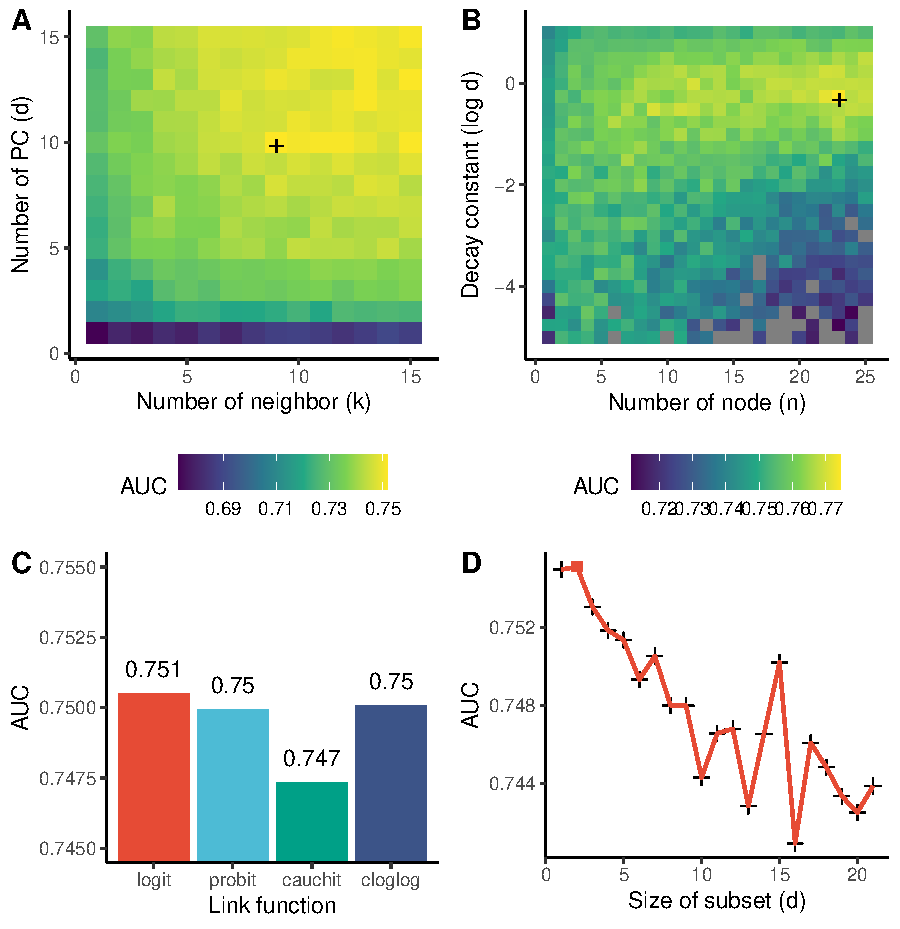
\includegraphics[width=0.7\linewidth]{tune.pdf}
  \caption{\small\textbf{A} KNN의 hyperparameter tuning 결과. 이웃의 수 $k=1,\,\cdots,\,15$와 주성분의 개수 $d=1,\,\cdots,\,15$에 대해 grid search를 수행하였으며 KNN은 각각의 피실험체에 대해 적합하였다. 5번의 10-fold CV를 통해 계산된 AUC의 최댓값은 $k=9$과 $d=10$인 경우($\mathrm{AUC}=0.752$)에 얻어졌다 (검은색 +). \textbf{B} ANN의 hyperparameter tuning 결과. 노드의 개수 $n=1,\,\cdots,\,25$과 decay constant $d=e^{1-0.25i}$ ($i=0,\,\cdots,\,24$)에 대해 grid search를 수행하으며 피실험체를 indicator variable로 하여 ANN을 적합하였다. 5번의 10-fold CV를 통해 계산된 AUC의 최댓값은 $n=23$과 $d=e^{-0.25}$인 경우($\mathrm{AUC}=0.775$)에 얻어졌다 (검은색 +). \textbf{C} 로지스틱 회귀의 link tuning 결과. Logit, probit, cauchit, complementary log-log(cloglog)에 대해 피실험체를 indicator variable로 하여 로지스틱 회귀모형을 적합하였다. 최초의 full model은 AIC를 기준으로 stepwise 모형 선택을 거쳤으며, 그 결과 선택된 모형으로 5번의 10-fold CV를 수행하고 AUC를 구하였다. AUC의 최댓값은 logistic link를 사용한 경우($\mathrm{AUC}=0.751$)에 얻어졌다. \textbf{D} Random forest의 hyperparameter tuning 결과. 개별 결정트리 적합시 사용할 변수의 수 $d=1,\,\cdots,\,21$에 대해 grid search를 수행하였다. 5번의 10-fold CV를 통해 계산된 AUC의 최댓값은 $d=2$인 경우($\mathrm{AUC}=0.755$)에 얻어졌다 (빨간색 네모).}
  \label{fig:tune}
\end{figure}

\paragraph{Naive Bayes} 
\texttt{Naive Bayes} 분류기는 각 변량이 서로 독립적이라는 다소 극단적인 가정 하에 베이즈 분류기를 계산하여 얻는 분류기이다. 그 이름에서 알 수 있듯이 관측한 표본으로부터 조건부확률을 계산하여 이를 분류에 이용하며, 고전적인 분류기 중에서도 단순한 분류기에 속한다. 본 연구에서는 \texttt{R} 함수 \textit{naiveBayes}(\texttt{e1071} 패키지)를 이용하여 적합하였다.

\paragraph{LDA} 

\texttt{LDA}(\texttt{Linear Discriminant Anlaysis}; 선형판별분석)은 두 그룹이 각각 다변량 정규분포를 따른다고 그룹간의 분산이 같다는 가정 하에 베이즈 분류기를 계산하여 얻는 분류기이다. 그 계산과정에서 두 그룹간의 분산은 최대화되고 그룹 내의 분산은 최소화하는 방향을 찾아 자료를 해당 방향으로 사영한다는 점에서 \texttt{PCA}와 그 아이디어가 유사하다. 본 연구에서는 \texttt{R} 함수 \textit{lda}(\texttt{MASS} 패키지)를 이용하여 적합하였다.

\paragraph{KNN}

\texttt{KNN}(\texttt{$k$-Nearest Neighbor}; $k$ 최근접 이웃 알고리즘)은 분류 알고리즘으로, 새로운 관측값 $\mathbf{x}\in\mathbb{R}^p$에 대해 이와 가장 가까운 $k$개의 관측값(이웃)이 어느 그룹에 속하는지 살펴 다수결에 따라 $\mathbf{x}$를 분류한다. 이론적으로 이는 관측값이 충분히 조밀하다는 가정 하에 베이즈 분류기의 근사가 된다. 본 연구에서는 \texttt{R} 함수 \textit{knn}(\texttt{class} 패키지)을 이용하였다.

자료가 고차원인 경우에는 차원의 저주에 의해 거리의 의미가 약해지므로 \texttt{PCA}와 같은 차원축소를 거친 자료를 이용하는 것이 바람직하다 \texttt{\citep{beyer1999nearest}}. 본 연구에서는 앞서 수행한 \texttt{PCA} 결과를 사용하였고, 10-\texttt{fold CV}를 통해 계산한 \texttt{AUC}를 기준으로 이웃의 수 $k$와 사용할 주성분의 개수 $d$를 결정하였다. 그림 \ref{fig:tune}의 A는 \texttt{hyperparameter tuning} 결과를 나타낸 것으로, 9개의 이웃과 10개의 주성분을 사용할 때 \texttt{AUC}를 기준으로 가장 좋은 예측력을 보였다.

\paragraph{ANN}

\texttt{ANN}(\texttt{Artificial Neural Network}; 인공신경망)은 근래 큰 인기를 끌고 있는 비모수적인 분류기로 인간의 뇌를 모방하여 개개의 뉴런들과 각 뉴런의 활성함수가 합쳐져 동작한다. \texttt{ANN}은 사용되는 분야에 따라 다양한 형태와 변형들이 존재하는데, 본 연구에서는 가장 단순한 형태인 \texttt{single layer FFNN}(\texttt{FeedFoward Neural Network})를 사용하였다. 이론적으로 \texttt{ANN}은 비선형회귀의 일종으로, 아핀 변환의 합성으로 표현된다. 특히 \texttt{single layer FFNN}의 경우 \texttt{universal approximation theorem}에 의해 적절한 조건을 만족하는 어느 함수든 원하는 만큼 근사할 수 있음이 알려져 있다 \texttt{\citep{leshno1993multilayer}}.

본 연구에서는 \texttt{R} 함수 \textit{nnet}(\texttt{nnet} 패키지)을 이용하여 적합하였는데, 각 노드의 가중치 최적화를 위해 \texttt{CE}(\texttt{Cross-Entropy}) 손실함수를 사용하였다. 한편, \texttt{ANN}은 자료에 과적합되는 경향이 있다. 복잡한 구조 속에서 네트워크가 원래의 자료를 그냥 외워버리는 것이다. 이를 방지하기 위해 가중치 최적화를 위한 반복 중에 의도적으로 적합을 방해하는 \texttt{decay constant} $d$를 도입한다. 본 연구에서는 10-\texttt{fold CV}를 통해 계산한 \texttt{AUC}를 기준으로 \texttt{decay constant} $d$와 은닉층의 노드 개수 $n$을 결정하였다. 그림 \ref{fig:tune}의 B는 \texttt{hyperparameter tuning} 결과를 나타낸 것으로, 23개의 노드와 \texttt{decay constant} $e^{-0.25}$를 사용할 때 \texttt{AUC}를 기준으로 가장 좋은 예측력을 보였다.

\paragraph{로지스틱 회귀}

로지스틱 회귀는 기존 신경과학계의 접근방식대로 반복측정으로 인한 자료의 종속성을 고려하지 않고, 이가 모두 독립하는 가정 하에 사용할 수 있는 분류기이다. 이러한 독립성의 고려를 제외하면 베르누이 분포의 모수를 \texttt{link} 함수로 설명변수의 선형결합과 연관짓는 다는 점은 \texttt{GLMM}과 그 아이디어가 동일하다. 다만, 로지스틱 회귀를 이용한 분류는 두 그룹이 이미 잘 분류되어 있는 경우에 이를 적합하는 \texttt{IRLS} (\texttt{Iteratively Reweighted Least Squares}) 알고리즘이 수치적으로 불안정해진다는 단점이 있는데, 앞서 \texttt{PCA}를 통해 확인한 바와 같이 본 연구에서 다루는 자료에서는 \texttt{Hit}과 \texttt{Miss} 두 그룹이 잘 섞여 있으므로 이는 크게 문제되지 않을 것이다.

이때 \texttt{link} 함수로는 앞서 사용한 \texttt{logit link} 외에 \texttt{probit}, \texttt{cauchit}, \texttt{complementary log-log} 등의 다양한 함수를 사용할 수 있다. (표 \ref{tab:logistic_link} 참조) 본 연구에서는 각각의 \texttt{link} 함수에 대해 \texttt{AIC}를 기준으로 \texttt{stepwise} 모형 선택을 진행하여 최적의 모형을 탐색한 후, 10-\texttt{fold CV}를 통해 계산한 \texttt{AUC}를 기준으로 최종적으로 사용할 \texttt{link} 함수를 결정하였다. 본 연구에서는 \texttt{R} 함수 \textit{glm}을 이용하여 모형을 적합하고, \texttt{R} 함수 \textit{stepAIC}(\texttt{MASS} 패키지)를 이용하여 \texttt{stepwise} 모형 선택을 수행하였다. 그림 \ref{fig:tune}의 \texttt{C}는 이상의 방식으로 구한 \texttt{link} 함수 별 \texttt{AUC}를 나타낸 것으로 \texttt{logit link}를 사용할 때 \texttt{AUC}를 기준으로 가장 좋은 예측력을 보였다.

\begin{table}[tp]
  \linespread{1}
  \renewcommand{\familydefault}{\sfdefault}\normalfont
  \centering
  \caption{\bf 로지스틱 회귀에서의 link 함수}
  \begin{tabularx}{\linewidth}{XX}
  \hline
  \header 이름 & 정의\\
  \hline
  Logit link & $g(x)=\log(x/(1-x))$\\
  Probit link & $g(x)=\Phi^{-1}(x)$ $^a$\\
  Cauchit link & $g(x)=\tan(\pi(x-1/2))$ $^b$\\
  Complementary log-log & $g(x)=\log(-\log(1-x))$\\
  \hline
  \end{tabularx}
  \begin{flushleft}
    \footnotesize $^a$ $\Phi$: 표준정규분포함수의 누적분포함수\\
    $^b$ 이는 $t(1)$ 분포(\texttt{Cauchy} 분포)의 누적분포함수의 역함수이다.
  \end{flushleft}
  \label{tab:logistic_link}
\end{table}

\paragraph{Random forest}

\texttt{Random forest}는 여러 개의 결정트리를 적합한 뒤, 각 트리의 예측 결과를 종합하여 최종 예측치를 결정하는 앙상블 기법의 일종이다. 이때, 각각의 결정트리는 전체 변량 중의 몇개의 부분집합만을 이용하여 적합되며, 같은 부분집합을 사용하더라도 각 트리의 적합 과정에서 최대 허용 깊이 등의 \texttt{hyperparameter}를 다르게 설정하여 전체 \texttt{forest}가 랜덤성을 띄도록 한다. 이는 과적합의 문제를 막기 위한 것이다.

본 연구에서는 \texttt{R} 함수 \textit{randomForest}(\texttt{randomForest} 패키지)를 이용하여 적합하였다. 이때, \texttt{forest}를 구성하는 결정트리의 수는 충분히 많아야 하므로 \textit{randomForest} 함수의 기본값인 500개로 설정하였다. 한편, 각 트리의 적합에 있어 사용할 변량의 부분집합의 크기 $d$는 \texttt{random forest}의 성능에 영향을 주는 중요한 \texttt{hyperparameter}이므로 10-\texttt{fold CV}를 통해 계산한 \texttt{AUC}를 기준으로 결정하였다. 그림 \ref{fig:tune}의 \texttt{D}는 \texttt{hyperparameter tuning} 결과를 나타낸 것으로, 변량의 부분집합의 크기가 2일때 \texttt{AUC}를 기준으로 가장 좋은 예측력을 보였다.

이상의 분류기들을 적합하여 각각 100번의 10-\texttt{fold CV}를 수행하여 \texttt{AUC}, \texttt{F score}, \texttt{MCC}를 계산하였다. 이와 더불어 다음과 같이 정의되는 \texttt{TPR}(\texttt{True Positive Rate}), \texttt{TNR}(\texttt{True Negative Rate}), \texttt{ACC}(\texttt{Accuracy}) 또한 계산하였다.
\begin{align}
  \mathrm{TPR}&=\frac{\mathrm{TP}}{\mathrm{TP}+\mathrm{FN}}\\
  \mathrm{TNR}&=\frac{\mathrm{TN}}{\mathrm{TN}+\mathrm{FP}}\nonumber\\
  \mathrm{ACC}&=\frac{\mathrm{TP}+\mathrm{TN}}{\mathrm{TP}+\mathrm{FN}+\mathrm{TN}+\mathrm{FP}}\nonumber
\end{align}

\section{결과}

\begin{figure}[tp]
  \renewcommand{\familydefault}{\sfdefault}\normalfont
  \centering
  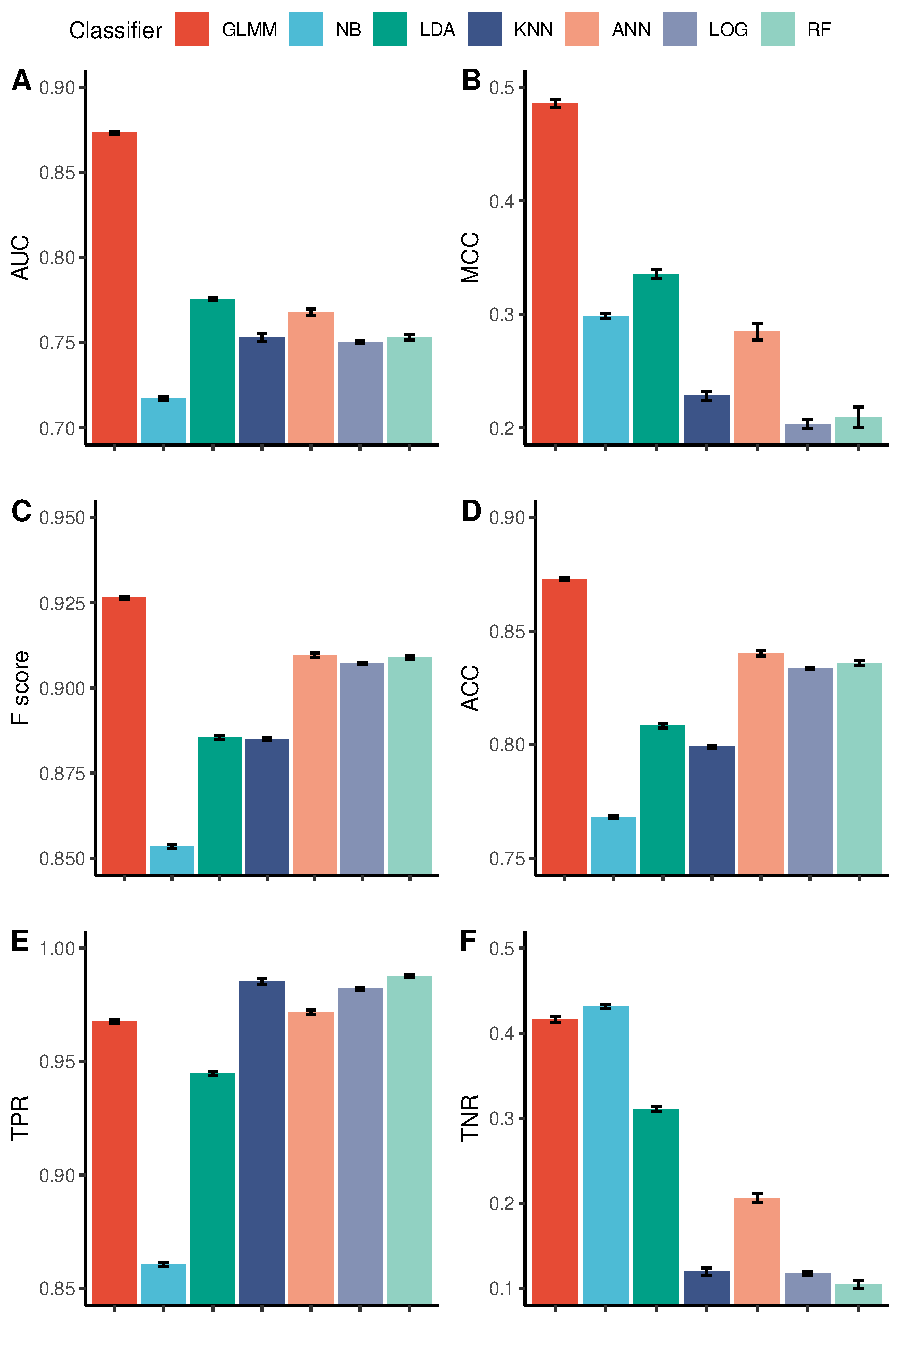
\includegraphics[width=0.7\linewidth]{Rplot.pdf}
  \caption{\small GLMM, naive Bayes, LDA, KNN, ANN, 로지스틱 회귀, random forest의 CV 결과. 100번의 10-fold CV를 통해 계산한 \textbf{A} AUC, \textbf{B} MCC, \textbf{C} F score, \textbf{D} ACC, \textbf{E} TPR, \textbf{F} TNR을 나타냈다. 에러바는 1sd를 의미한다. GLMM, ANN, 로지스틱 회귀, random forest는 피실험체를 indicator variable로 하여 하나의 모형을 적합했고, naive Bayes, LDA, KNN는 피실험체별로 하나씩의 모형을 적합했다.}
  \label{fig:cv}
\end{figure}

그림 \ref{fig:cv}는 \texttt{CV} 결과를 나타낸 것으로 \texttt{AUC}, \texttt{MCC}, \texttt{F score}, \texttt{ACC} 모두 \texttt{GLMM}이 다른 분류기에 비해 우수함을 확인할 수 있다. 특히, \texttt{TPR}과 \texttt{TNR}을 보면, 다른 분류기가 그 비율이 많은 \texttt{Hit} 그룹으로 다소 편향되게 예측하는 것에 비하여 \texttt{GLMM}은 두 그룹간의 불균형에도 불구하고 그 경계를 비교적 잘 구분하고 있음을 알 수 있다.

\begin{table}[tp]
  \linespread{1}
  \renewcommand{\familydefault}{\sfdefault}\normalfont
  \centering
  \caption{\bf GLMM 적합 결과 (고정효과)}
  \begin{tabularx}{\linewidth}{XXXXX}
  \hline
  \header 설명변수 & 계수 & 표준편차 & LRT $\Lambda$ & p-value\\
  \hline
  절편 & -4.766 & 0.608 & - & -\\
  \ACL delta & -0.030 & 0.082 & 4.304 & 1.68e-5 ***\\
  \ACL gamma & -0.191 & 0.136 & -0.393 & 0.694\\
  \ACL high gamma & -0.686 & 0.179 & -3.233 & 1.22e-3 **\\
  \ACR delta & 0.061 & 0.094 & 4.304 & 1.68e-5 ***\\
  \ACR theta & -0.038 & 0.138 & 4.304 & 1.68e-5 ***\\
  \ACR beta & 0.013 & 0.138 & 1.434 & 0.152\\
  \ACR gamma & -0.162 & 0.137 & -2.171 & 0.030 *\\
  \ACR high gamma & -0.645 & 0.199 & -0.478 & 0.633\\
  \PFCL delta & -0.255 & 0.075 & 0.075 & 1.77e-5 ***\\
  \PFCL theta & 0.065 & 0.115 & 0.115 & 1.77e-5 ***\\
  \PFCL beta & 0.556 & 0.119 & 0.119 & 8.12e-4 ***\\
  \PFCL gamma & -0.317 & 0.097 & -2.335 & 0.020 *\\
  \PFCL high gamma & 0.620 & 0.816 & -2.335 & 0.020 *\\
  \PPCL delta & 0.269 & 0.079 & 4.144 & 3.42e-5 ***\\
  \PPCL theta & 0.184 & 0.143 & -1.967 & 0.049 *\\
  \PPCL beta & 0.556 & 0.142 & 4.055 & 5.02e-5 ***\\
  \PPCL high gamma & -0.980 & 0.184 & -5.420 & 5.96e-8 ***\\
  \hline
  \end{tabularx}
  \label{tb:glmm_fixed}
\end{table}

\begin{table}[tp]
  \linespread{1}
  \renewcommand{\familydefault}{\sfdefault}\normalfont
  \centering
  \caption{\bf GLMM 적합 결과 (랜덤효과)}
  \begin{tabularx}{\linewidth}{XXXX}
  \hline
  \header 그룹 & 설명변수 & 분산 & 표준편차\\
  \hline
  피실혐체별 세션 & 절편 & 2.72050 & 1.6494\\
  피실험체 & 절편 & 0.01301 & 0.1141\\
  \hline
  \end{tabularx}
  \label{tb:glmm_rand}
\end{table}

\texttt{GLMM} 모형을 적합한 결과는 표 \ref{tb:glmm_fixed}, \ref{tb:glmm_rand}과 같다. 적합 결과를 보면, 우선 랜덤효과에서 피실험체 수준의 오차의 분산이 거의 0임을 알 수 있다. 이는 피실험체 수준의 오차보다 반복측정에 있어서의 개개의 세션에서의 오차가 지배적임을 함의한다. 다만, 사실은 피실험체 수준의 변동성이 세션 수준의 변동성으로 고려되어 적합되었을 가능성이 있으므로 섣불리 피실험체가 서로 동일하다고 결론지어서는 안될 것이다. 고정효과를 보면, \texttt{\PFCL}과 \texttt{\PPCL} 부위의 다양한 주파수대에 걸쳐 해당 \texttt{bandpower}가 피실험체의 행동 결과에 유의한 영향을 주고 있음을 알 수 있다. 그러나 그 방향성은 제각각인데, 예컨대 \texttt{\PPCL}의 \texttt{delta bandpower}와 \texttt{beta bandpower}는 \texttt{Hit}의 확률과 양의 상관을 가지는 방향으로 유의하고, 동일한 부위의 \texttt{high gamma bandpower}는 \texttt{Hit}의 확률과 음의 상관을 가지는 방향으로 유의하다.

\section{코드 및 분석도구}
이상 채널 제거와 \texttt{LFP} 정규화, \texttt{bandpower} 계산은 \texttt{MATLAB}으로 하였다. 나머지 분석은 모두 \texttt{R}로 하였다. 분석에 사용한 코드는 \texttt{github} \url{https://github.com/eik4862/GLMM}에서 찾아볼 수 있다.

\section{Acknowledgement}
본 연구에서 사용한 자료는 한국과학기술연구원 신경과학연구단의 한효빈, 이가은, 최지현이 실험을 통해 얻은 것으로 3/2/2020 허락을 받고 사용하였다. 동물 실험에 대한 규정 준수 및 관련된 자세한 사항은 \texttt{\cite{han2019functional}} 참조.

\section{Technicality}

\subsection{라플라스 근사를 이용한 GLMM의 로그가능도 근사}

본 절에서는 \texttt{GLMM}의 로그가능도인 
\begin{align}\label{eq:GLMMloglik}
  l(\beta,\,\Psi)&=\log\int_{\mathbb{R}^q}\exp\bigg(\sum_{i=1}^n[\mathbf{z}_i'\gamma Y_i-A(\mathbf{x}_i'\beta+\mathbf{z}_i'\gamma)]-\frac{\gamma'\Psi^{-1}\gamma}{2}\bigg)\,d\gamma\nonumber\\
  &\qquad\qquad\qquad-\frac{1}{2}\log\det\Psi+\sum_{i=1}^n\mathbf{x}_i'\beta Y_i+\mathrm{const.}
\end{align}
를 라플라스 근사를 통해 수치적으로 계산하는 구체적인 방법에 대해 알아본다. 이는 본 연구에서 \texttt{GLMM}의 적합에 사용된 \texttt{R} 함수 \textit{glmer}(\texttt{lme4} 패키지)에서 모형을 적합할 때 적용되는 수치적분법이다. 먼저 적분에 대한 라플라스 근사의 \texttt{justification}을 위해 다음 정리를 증명한다.\\

\noindent\textsf{\textbf{정리} 원점 $\mathbf{0}$ 근방에서 각각 $\mathcal{C}^1$급이고 $\mathcal{C}^2$급인 함수 $f,\,g:\mathbb{R}^d\to\mathbb{R}$에 대해 $f(\mathbf{0})>0$이고 $\nabla^2g(\mathbf{0})>0$이라 하자. 나아가, 임의의 $\delta>0$에 대해 적당한 $\rho>0$가 존재하여 $||\mathbf{x}||\geq\delta$이면 $g(\mathbf{x})-g(\mathbf{0})\geq\rho$라 하자. 만약 적당한 $a_0\in\mathbb{R}$가 존재하여 임의의 $a\geq a_0$에 대해 적분 $\int_{\mathbb{R}^d}fe^{-ag}\,d\mu$가 절대수렴한다면, $a\to\infty$ 일 때
\begin{equation}
  \int_{\mathbb{R}^d}fe^{-ag}\,d\mu\bigg/\bigg[f(\mathbf{0})e^{-ag(\mathbf{0})}\bigg(\frac{2\pi}{a}\bigg)^{d/2}\frac{1}{\sqrt{\det\nabla^2g(\mathbf{0})}}\bigg]\to1
\end{equation}
이 성립한다. 여기서 $\mu$는 르벡측도이다.}

\proof 필요하다면 분자와 분모에 $e^{ag(\mathbf{0})}$을 곱하고 $g$ 대신 $g-g(\mathbf{0})$을 생각하여 \texttt{WLOG}, $g(\mathbf{0})=0$이라 해도 된다. 이제 테일러 근사로부터 $\mathbf{x}\to\mathbf{0}$이면 $\nabla g(\mathbf{x})=\nabla^2g(\mathbf{0})\mathbf{x}+o(||\mathbf{x}||)$이고 로피탈의 법칙으로부터 $\mathbf{x}\to\mathbf{0}$이면 $g(\mathbf{x})-\mathbf{x}'\nabla^2g(\mathbf{0})\mathbf{x}/2=o(||\mathbf{x}||^2)$임을 안다. 한편, $f$가 $\mathbf{0}$에서 $\mathcal{C}^1$급이고 $f(\mathbf{0})>0$임을 생각하면 충분히 작은 임의의 $\epsilon>0$에 대해 적당한 $\delta>0$가 존재하여 $||\mathbf{x}||<\delta$이면
\begin{align}
  (1-\epsilon)f(\mathbf{0})\leq f(\mathbf{x})\leq(1+\epsilon)f(\mathbf{0})\\
  -\epsilon||\mathbf{x}||^2\leq g(\mathbf{x})-\frac{1}{2}\mathbf{x}'\nabla^2g(\mathbf{0})\mathbf{x}\leq \epsilon ||\mathbf{x}||^2
\end{align}
임을 안다.

이제 적분의 범위를 나누어 $\mathbb{R}^d\setminus B(\mathbf{0},\,\delta)$에서 적분의 기여를 생각하면, 주어진 $g$에 대한 조건으로부터 $a\geq a_0$이면 
\begin{align}
  \bigg|\int_{\mathbb{R}^d\setminus B(\mathbf{0},\,\delta)}fe^{-ag}\,d\mu\bigg|&\leq\int_{\mathbb{R}^d\setminus B(\mathbf{0},\,\delta)}|f|e^{-(a-a_0)g}e^{-a_0g}\,d\mu\\
  &\leq e^{-(a-a_0)\rho}\int_{\mathbb{R}^d}|f|e^{-a_0g}\,d\mu\nonumber
\end{align}
에서 $\int_{\mathbb{R}^d\setminus B(\mathbf{0},\,\delta)}fe^{-ag}\,d\mu=O(e^{-a\rho})$이다. 한편, $B(\mathbf{0},\,\delta)$에서는
\begin{align}
  \int_{B(\mathbf{0},\,\delta)}fe^{-ag}\,d\mu&\leq(1+\epsilon)f(\mathbf{0})\int_{\mathbb{R}} \exp\bigg(-\frac{a}{2}\mathbf{x}'[\nabla^2g(\mathbf{0})-2\epsilon I_d]\mathbf{x}\bigg)\,d\mu(\mathbf{x})\nonumber\\
  &=(1+\epsilon)f(\mathbf{0})\bigg(\frac{2\pi}{a}\bigg)^{d/2}\frac{1}{\sqrt{\det(\nabla^2 g(\mathbf{0})-2\epsilon I_d)}}\nonumber
\end{align}
으로 위로 유계이다. 이로부터
\begin{equation}
  \limsup_{a\to\infty}a^{d/2}\int_{\mathbb{R}}fe^{-ag}\,d\mu\leq(1+\epsilon)f(\mathbf{0})\frac{(2\pi)^{d/2}}{\sqrt{\det(\nabla^2 g(\mathbf{0})-2\epsilon I_d)}}\nonumber
\end{equation}
이고 $\epsilon$이 임의의 양수라는 점을 떠올리면
\begin{equation}\label{eq:limsup}
  \limsup_{a\to\infty}a^{d/2}\int_{\mathbb{R}}fe^{-ag}\,d\mu\leq f(\mathbf{0})\frac{(2\pi)^{d/2}}{\sqrt{\det\nabla^2 g(\mathbf{0})}}
\end{equation}
을 얻는다.

한편, 적당한 $\lambda>0$가 존재하여 $||\mathbf{x}||\geq\delta$이면 $\mathbf{x}'[\nabla^2g(\mathbf{0})/2+\epsilon I_d]\mathbf{x}\geq\lambda$이고 모든 $a>0$에 대해 
\begin{equation}
  \int_{\mathbb{R}^d}\exp\bigg(-\frac{a}{2}\mathbf{x}'[\nabla^2g(\mathbf{0})+2\epsilon I_d]\mathbf{x}\bigg)\,d\mu(\mathbf{x})<\infty
\end{equation}
이므로 앞선 논의와 비슷하게 하면 $\int_{\mathbb{R}^d\setminus B(\mathbf{0},\,\delta)}\exp(-a\mathbf{x}'[\nabla^2g(\mathbf{0})+2\epsilon I_d]\mathbf{x}/2)\,d\mu(\mathbf{x})=O(e^{-a\lambda})$임을 안다. 이로부터
\begin{align}
  (1&-\epsilon)f(\mathbf{0})\int_{B(\mathbf{0},\,\delta)}\exp\bigg(-\frac{a}{2}\mathbf{x}'[\nabla^2g(\mathbf{0})+2\epsilon I_d]\mathbf{x}\bigg)\,d\mu(\mathbf{x})\\
  &\geq(1-\epsilon)f(\mathbf{0})\int_{\mathbb{R}^d}\exp\bigg(-\frac{a}{2}\mathbf{x}[\nabla^2g(\mathbf{0})+2\epsilon I_d]\mathbf{x}\bigg)\,d\mu(\mathbf{x})-O(e^{-a\lambda})\nonumber\\
  &=(1-\epsilon)f(\mathbf{0})\bigg(\frac{2\pi}{a}\bigg)^{d/2}\frac{1}{\sqrt{\det(\nabla^2 g(\mathbf{0})+2\epsilon I_d)}}+O(e^{-a\lambda})\nonumber
\end{align}
이고, 곧 
\begin{equation}
  \liminf_{a\to\infty}a^{d/2}\int_{\mathbb{R}^d}fe^{-ag}\,d\mu\geq(1-\epsilon)f(\mathbf{0})\frac{(2\pi)^{d/2}}{\sqrt{\det(\nabla^2 g(\mathbf{0})+2\epsilon I_d)}}
\end{equation}
에서 $\epsilon$이 임의의 양수라는 점을 떠올리면
\begin{equation}\label{eq:liminf}
  \liminf_{a\to\infty}a^{d/2}\int_{\mathbb{R}^d}fe^{-ag}\,d\mu\geq f(\mathbf{0})\frac{(2\pi)^{d/2}}{\sqrt{\det\nabla^2 g(\mathbf{0})}}
\end{equation}
을 얻는다. 이제 식 \ref{eq:limsup}과 \ref{eq:liminf}로부터 증명이 끝난다.\hfill$\blacksquare$\\

이로부터 적분 $\int_{\mathbb{R}^d}fe^{-ag}\,d\mu$를
\begin{equation}
  f(\mathbf{0})e^{-ag(\mathbf{0})}\bigg(\frac{2\pi}{a}\bigg)^{d/2}\frac{1}{\sqrt{\det\nabla^2g(\mathbf{0})}}
\end{equation}
으로 근사할 수 있다. 한편, 라플라스 근사의 오차를 줄이기 위해서는 함수 $g$의 \texttt{mass}가 $\mathbf{0}$ 근처에 집중되어 있어야 하므로 평행이동을 통해 $g$가 $\mathbf{0}$에서 최댓값을 가지도록 조정한 후에 근사하는 것이 일반적이다. 이를 \texttt{GLMM}의 로그가능도(식 \ref{eq:GLMMloglik})에 적용하기 위해 함수
\begin{equation}
  \gamma\mapsto\sum_{i=1}^n[A(\mathbf{x}_i'\beta+\mathbf{z}_i'\gamma)-\mathbf{z}_i'\gamma Y_i]+\frac{\gamma'\Psi^{-1}\gamma}{2}
\end{equation}
가 $\gamma_*\in\mathbb{R}^q$에서 최댓값을 가진다고 하자. 그렇다면 평행이동을 통해 \texttt{GLMM}의 로그가능도에서의 적분은 다음과 같이 쓸 수 있다.
\begin{equation}
  \int_{\mathbb{R}^q}\exp\bigg(\sum_{i=1}^n[\mathbf{z}_i'(\gamma+\gamma_*)Y_i-A(\mathbf{x}_i'\beta+\mathbf{z}_i'(\gamma+\gamma_*))]-\frac{(\gamma+\gamma_*)'\Psi^{-1}(\gamma+\gamma_*)}{2}\bigg)\,d\gamma
\end{equation}
라플라스 근사로부터 위의 적분은
\begin{equation}
  \exp\bigg(-\sum_{i=1}^nA(\mathbf{x}_i'\beta)\bigg)\frac{(2\pi)^{d/2}}{\sqrt{\det(\sum_{i=1}^nA''(\mathbf{x}_i'\beta+\mathbf{z}_i'\gamma_*)\mathbf{z}_i\mathbf{z}_i'+\Psi^{-1})}}
\end{equation}
로 근사할 수 있으므로 곧 식 \ref{eq:GLMMloglik}를 최대화하는 것은 근사적으로
\begin{equation}
  -\sum_{i=1}^nA(\mathbf{x}_i'\beta)-\frac{1}{2}\log\det\bigg(\sum_{i=1}^nA''(\mathbf{x}_i'\beta+\mathbf{z}_i'\gamma_*)\mathbf{z}_i\mathbf{z}_i'+\Psi^{-1}\bigg)-\frac{1}{2}\log\det\Psi+\sum_{i=1}^n\mathbf{x}_i'\beta Y_i
\end{equation}
를 $\beta,\,\Psi$에 대해 최대화하는 것과 같다.

\subsection{GLMM의 고정효과에 대한 검정통계량의 극한분포}

본 절에서는 \texttt{GLMM}의 고정효과에 대한 선형가설
\begin{equation}\label{eq:linearHypo}
  H_0:T\beta=\xi\qquad H_1:T\beta\ne\xi\qquad(\mathrm{rk}\,T=r<p)
\end{equation}
을 검정하는 \texttt{LRT} 검정통계량
\begin{equation}
  \Lambda=-2[l(\widehat{\beta},\,\widehat{\psi})-l(\widetilde{\beta},\,\widetilde{\psi})]
\end{equation}
의 극한분포가 $\chi^2(p-r)$임을 보이도록 한다. 이를 위해 보다 일반적인 다음 정리를 증명한다.\\

\noindent\textsf{\textbf{정리} 모형 $\mathcal{P}=\{\mathbf{P}_\theta\}_{\theta\in\Theta}$이 $\vartheta\in\Theta^\circ\subseteq\mathbb{R}^d$에 대해 differentiable in quadratic mean\footnote{모형 $\mathcal{P}=\{\mathbf{P}_\theta\}_{\theta\in\Theta}$이 \texttt{differentiable in quadratic mean}이라 함은 임의의 $\theta\in\Theta$에 대해 확률측도 $\mathbf{P}_\theta$의 확률밀도함수 $p_\theta$에 대해 적당한 가측함수 $\dot{l}_\theta:\mathbb{R}\to\mathbb{R}^d$이 존재하여 $\mathbf{h}\to\mathbf{0}$일 때
\begin{equation}
  \int_{\mathbb{R}}\,\bigg(\sqrt{p_{\theta+\mathbf{h}}}-\sqrt{p_{\theta}}-\frac{1}{2}\mathbf{h}'\dot{l}_\theta\sqrt{p_\theta}\bigg)^2d\mu=o(||\mathbf{h}||^2)
\end{equation}
임을 의미한다.}이고 Fisher 정보행렬 $I_{\vartheta}$가 가역이라 하자. 이제 가설
\begin{equation}
  H_0:\theta\in\Theta_0\qquad H_1:\theta\in\Theta_1\qquad(\Theta_0\sqcup\Theta_1=\Theta)
\end{equation}
를 검정하는 상황을 생각하고, 적당한 $L^2(\mathbf{P}_{\vartheta})$ 함수 $\dot{l}:\mathbb{R}\to\mathbb{R}$이 존재하여 임의의 $x\in\mathbb{R}$와 $\vartheta$의 근방 $\mathcal{N}\subseteq\Theta$에 속하는 임의의 $\theta_1,\,\theta_2\in\mathcal{N}$에 대해
\begin{equation}
  |\log p_{\theta_1}(x)-\log p_{\theta_2}(x)|\leq\dot{l}(x)||\theta_1-\theta_2||
\end{equation}
라 하자. 여기서 $p_\theta$는 확률측도 $\mathbf{P}_\theta$의 확률밀도함수이다. 만약 $\theta$의 MLE $\widehat{\theta}_n$과 귀무가설 하에서의 MLE $\widetilde{\theta}_n$에 대해 $\widehat{\theta}_n,\,\widetilde{\theta}_n\stackrel{\mathbf{P}_{\vartheta}}{\to}\theta_0$이며 집합 $H_n=\sqrt{n}(\Theta-\vartheta),\,H_n^0=\sqrt{n}(\Theta_0-\vartheta)\subseteq\mathbb{R}^d$가 각각 집합 $H,\,H^0\subseteq\mathbb{R}^d$으로 수렴하면\footnote{집합 $A_n\subseteq\mathbb{R}^d$이 $A\subseteq\mathbb{R}^d$로 수렴한다 함은 임의의 수열 $a_n\in A_n$에 대해 $a_n\to a$이면 $a\in A$이고, 나아가 이의 임의의 부분열 $\{a_{n_i}\}$에 대해 $a_{n_i}\to a_*$이면 $a_*\in A$임을 의미한다.} LRT의 검정통계량 $\Lambda_n=-2[l(\widetilde{\theta}_n)-l(\widehat{\theta}_n)]$에 대해
\begin{equation}
  \Lambda_n\stackrel{\mathbf{P}_{\vartheta+\mathbf{h}/\sqrt{n}}}{\Rightarrow}||I_{\vartheta}^{1/2}\mathbf{Z}-I_{\vartheta}^{1/2}H^0||^2-||I_{\vartheta}^{1/2}\mathbf{Z}-I_{\vartheta}^{1/2}H||^2
\end{equation}
이 성립한다.\footnote{집합 $A\subseteq\mathbb{R}^d$와 점 $\mathbf{x}\in\mathbb{R}^d$에 대해 $||\mathbf{x}-A||$는 $\inf_{\mathbf{y}\in A}||\mathbf{x}-\mathbf{y}||$로 정의한다.} 여기서 $\mathbf{Z}\sim\mathbf{N}_d(\mathbf{0},\,I_\vartheta^{-1})$이다.}

\proof 검정하고자 하는 가설은 가설 $H_0:\mathbf{h}\in H_n,\,H_1:\mathbf{h}\in H_n^0$을 검정통계량
\begin{equation}
  \Lambda_n=2\sup_{\mathbf{h}\in H_n}\log\frac{\prod_{i=1}^np_{\vartheta+\mathbf{h}/\sqrt{n}}(X_i)}{\prod_{i=1}^np_{\vartheta}(X_i)}-2\sup_{\mathbf{h}\in H_n^0}\log\frac{\prod_{i=1}^np_{\vartheta+\mathbf{h}/\sqrt{n}}(X_i)}{\prod_{i=1}^np_{\vartheta}(X_i)}
\end{equation}
로 검정하는 것과 동등하다. 이제 \texttt{empirical probabiltiy measure} $\mathbb{P}_n$에 대해 \texttt{empirical process} $\mathbb{G}_n=\sqrt{n}(\mathbb{P}_n-\mathbf{P}_\vartheta)$를 생각하고, 확률과정 $\mathbb{Z}_n$를
\begin{equation}
  \mathbb{Z}_n(\mathbf{h})=n\int_{\mathbb{R}^n}\log\frac{p_{\vartheta+\mathbf{h}/\sqrt{n}}}{p_{\vartheta}}\,d\mathbb{P}_n-\mathbf{h}'\int_{\mathbb{R}^n}\dot{l}_\vartheta\,d\mathbb{G}_n+\frac{1}{2}\mathbf{h}'I_\vartheta\mathbf{h}
\end{equation}
로 정의하자. 여기서 $l_\vartheta=\log p_\vartheta$이며 $\dot{l}_\vartheta$는 $l_\vartheta$의 \texttt{differentiable in quadratic mean}의 의미로의 미분이다. 그렇다면 \texttt{\cite{van2000asymptotic}}의 정리 7.12의 증명으로부터 임의의 $M\geq0$에 대해
\begin{equation}\label{eq:uniformConv}
  \sup_{||\mathbf{h}||\leq M}|Z_n(\mathbf{h})|\stackrel{\mathbf{P}_\vartheta}{\to}0
\end{equation}이고 $\sqrt{n}(\widehat{\theta}_n-\vartheta),\,\sqrt{n}(\widetilde{\theta}_n-\vartheta)\stackrel{\mathbf{P}_\vartheta}{\to}0$임을 알 수 있다. 나아가, 위의 식 \ref{eq:uniformConv}가 충분히 천천히 $\infty$로 발산하는 임의의 수열 $\{M_n\}$에 대해서도 성립함을 쉽게 알 수 있다. 이러한 수열 $\{M_n\}$을 고정하면 앞선 결론으로부터 \texttt{MLE} $\widehat{\theta}_n$와 $\widetilde{\theta}_n$가 $B(\vartheta,\,M_n/\sqrt{n})$에 포함될 확률은 각각 1로 수렴하고, 따라서 $\Lambda_n$의 극한분포는 집합 $H_n$과 $H_n^0$을 각각 $H_n\cap B(\mathbf{0},\,M_n)$와 $H_n^0\cap B(\mathbf{0},\,M_n)$로 바꾸더라도 변함이 없다. 또한, 집합 $H_n\cap B(\mathbf{0},\,M_n)$와 $H_n^0\cap B(\mathbf{0},\,M_n)$이 각각 $H$와 $H^0$으로 수렴함도 자명하다. 이제 식 \ref{eq:uniformConv}으로부터 간단한 산수를 통해
\begin{align}
  \Lambda_n&=2\sup_{\mathbf{h}\in H_n}n\int_{\mathbb{R}^n}\log\frac{p_{\vartheta+\mathbf{h}/\sqrt{n}}}{p_{\vartheta}}\,d\mathbb{P}_n-2\sup_{\mathbf{h}\in H_n^0}n\int_{\mathbb{R}^n}\log\frac{p_{\vartheta+\mathbf{h}/\sqrt{n}}}{p_{\vartheta}}\,d\mathbb{P}_n\\
  &=2\sup_{\mathbf{h}\in H_n}\bigg(\mathbf{h}'\int_{\mathbb{R}^n}\dot{l}_\vartheta\,d\mathbb{G}_n-\frac{1}{2}\mathbf{h}'I_\vartheta\mathbf{h}\bigg)-2\sup_{\mathbf{h}\in H_n^0}\bigg(\mathbf{h}'\int_{\mathbb{R}^n}\dot{l}_\vartheta\,d\mathbb{G}_n-\frac{1}{2}\mathbf{h}'I_\vartheta\mathbf{h}\bigg)+o_{\mathbf{P}_\vartheta}(1)\nonumber\\
  &=\bigg|\bigg|I_\vartheta^{-1/2}\int_{\mathbb{R}^n}\dot{l}_\vartheta\,d\mathbb{G}_n-I_\vartheta^{1/2}H_0\bigg|\bigg|^2-\bigg|\bigg|I_\vartheta^{-1/2}\int_{\mathbb{R}^n}\dot{l}_\vartheta\,d\mathbb{G}_n-I_\vartheta^{1/2}H\bigg|\bigg|^2+o_{\mathbf{P}_\vartheta}(1)\nonumber
\end{align}
임을 안다. 마지막 등호는 \texttt{\cite{van2000asymptotic}}의 보조정리 7.13으로부터 성립하며, 여기서 $o_{\mathbf{P}_\vartheta}(1)$는 \texttt{little $o$ in probability}이다. 이제 \texttt{continuous mapping theorem}으로부터 증명이 끝난다.\hfill$\blacksquare$\\

\noindent\textsf{\textbf{보조정리} 확률벡터 $\mathbf{Z}\sim\mathbf{N}_d(0,\,I_d)$와 $\dim\mathsf{V}=k$인 부분공간 $\mathsf{V}<\mathbb{R}^d$에 대해 $||\mathbf{Z}-\mathsf{V}||^2\sim\chi^2(d-k)$이다.}

\proof 부분공간 $\mathsf{V}$의 기저를 $\beta$라 하고 이를 확장하여 $\mathbb{R}^d$의 기저를 구성하여 이를 $\gamma$라 하자. \texttt{WLOG}, $\gamma$의 첫 $k$개의 기저가 $\beta$라 하자. 그렇다면 임의의 $\mathbf{x}\in\mathbb{R}^d$에 대해 $||\mathbf{x}-\mathsf{V}||^2$는 $\gamma$를 기저로 할 때 $\mathbf{x}$ 좌표 $(x_1,\,\cdots,\,x_d)$를 사용하여 $\sum_{i=k+1}^dx_i^2$로 쓸 수 있다. 한편, $\mathbb{R}^d$의 표준기저 $\mathcal{E}$에서 $\gamma$로의 좌표변환을 기술하는 행렬 $I_{\mathcal{E}}^{\gamma}$는 직교행렬이므로 $\gamma$를 기저로 할 때 확률벡터 $\mathbf{Z}$의 좌표 $(Z_1,\,\cdots,\,Z_d)$에 대해 각 $Z_i$는 표준정규분포를 따른다. 이상의 사실을 종합하면 $||\mathbf{Z}-\mathsf{V}||^2=\sum_{i=k+1}^dZ_i^2\sim\chi^2(d-k)$이다.\hfill$\blacksquare$\\

먼저 $\xi=\mathbf{0}$인 경우를 생각하면 검정하고자 하는 가설(식 \ref{eq:linearHypo})은 $H_0:\beta\in \ker T$와 동등하고 $\dim\ker T=p-r$이다. 이 경우, \texttt{GLMM}이 위의 정리가 요구하는 조건을 모두 만족함을 쉽게 보일 수 있다 \texttt{\citep{van2000asymptotic}}. 그렇다면 이상의 논의로부터 $\Lambda$의 극한분포가 $\chi^2(p-r)$임을 알고, 일반적인 경우에는 적당한 $\beta_0\in T^{-1}(\xi)$에 대해 $\delta=\beta_0+\beta$의 \texttt{reparameterization}을 생각하면 같은 결론에 이른다.

동일한 가설을 검정하는 \texttt{Wald}의 검정통계량과 \texttt{Rao}의 검정통계량
\begin{align}
  W&=(T\widehat{\beta}-\xi)'\{T[\nabla^2_\beta l(\widehat{\beta},\,\widehat{\Psi})]^{-1}T'\}^{-1}(T\widehat{\beta}-\xi)\\
  R&=\nabla_\beta l(\widetilde{\beta},\,\widetilde{\Psi})'[\nabla^2_\beta l(\widetilde{\beta},\,\widetilde{\Psi})]^{-1}\nabla_\beta l\widetilde{\beta},\,\widetilde{\Psi})
\end{align}
의 경우, 로그가능도에 대한 테일러 근사로부터 $\Lambda=W+o_{\beta,\,\Psi}(1)=R+o_{\beta,\,\Psi}(1)$임을 보일 수 있고 \texttt{\citep{bickel2015mathematical}}, 따라서 두 검정통계량의 극한분포도 $\chi^2(p-r)$임을 안다.

\subsection{GLMM의 랜덤효과에 대한 예측값}

본 절에서는 \texttt{GLMM}에서 랜덤효과의 예측에 대한 \texttt{MSPE} $\mathbf{E}_{\beta,\,\Psi}||\gamma-\gamma_*||^2$가 $\mathbf{E}_{\beta,\,\Psi}(\gamma\vert\mathbf{Y})$의해 최소화됨을 보이도록 한다.\\

\noindent\textsf{\textbf{정리} 확률공간 $(\Omega,\,\mathcal{F},\,\mathbb{P})$와  확률벡터 $\mathbf{X}:\Omega\to\mathbb{R}^d$, sub-sigma field $\mathcal{E}\subseteq\mathcal{F}$를 생각하자. 그렇다면 임의의 $\mathcal{E}$-가측인 확률벡터 $\mathbf{Y}:\Omega\to\mathbb{R}^d$에 대해 $\mathbf{X},\,\mathbf{Y}\in L^2$라면 $\mathbf{E}([\mathbf{X}-\mathbf{E}(\mathbf{X}\vert\mathcal{E})]'\mathbf{Y})=0$이다.}

\proof 이는 $\mathbf{E}([\mathbf{X}-\mathbf{E}(\mathbf{X}\vert\mathcal{E})]'\mathbf{Y})=\mathbf{E}(\mathbf{E}([\mathbf{X}-\mathbf{E}(\mathbf{X}\vert\mathcal{E})]'\mathbf{Y}\vert\mathcal{E}))=\mathbf{E}(\mathbf{E}(\mathbf{X}-\mathbf{E}(\mathbf{X}\vert\mathcal{E})\vert\mathcal{E})'\mathbf{Y})=\mathbf{0}$에서 자명하다.\hfill$\blacksquare$\\

\noindent\textsf{\textbf{따름정리} 확률공간 $(\Omega,\,\mathcal{F},\,\mathbb{P})$와 확률벡터 $\mathbf{X}:\Omega\to\mathbb{R}^d$, sub-sigma field $\mathcal{E}\subseteq\mathcal{F}$에 대해 $\mathbf{X}\in L^2$라 하자. 그렇다면 $\argmin_{\mathbf{Y}\in L^2(\mathcal{E},\,\mathbb{P})}\mathbf{E}||\mathbf{X}-\mathbf{Y}||^2=\mathbf{E}(\mathbf{X}\vert\mathcal{E})$이다.}

\proof 임의의 $\mathbf{Y}\in L^2(\mathcal{E},\,\mathbb{P})$에 대해 $\mathbf{E}||\mathbf{X}-\mathbf{Y}||^2=\mathbf{E}||\mathbf{X}-\mathbf{E}(\mathbf{X}\vert\mathcal{E})||^2+\mathbf{E}||\mathbf{E}(\mathbf{X}\vert\mathcal{E})-\mathbf{Y}||^2+2\mathbf{E}((\mathbf{X}-\mathbf{E}(\mathbf{X}\vert\mathcal{E}))(\mathbf{E}(\mathbf{X}\vert\mathcal{E})-\mathbf{Y}))$인데 여기서 $\mathbf{E}(\mathbf{X}\vert\mathcal{E})-\mathbf{Y}\in L^2(\mathcal{E},\,\mathbb{P})$이므로 위의 정리로부터 $\mathbf{E}||\mathbf{X}-\mathbf{Y}||^2\geq\mathbf{E}||\mathbf{X}-\mathbf{E}(\mathbf{X}\vert\mathcal{E})||^2$이다. 증명은 이로써 충분하다.\hfill$\blacksquare$\\

이상의 결과로부터 \texttt{MSPE}를 최소화하는 $\gamma$의 예측값은 $\mathbf{E}_{\beta,\,\Psi}(\gamma\vert\mathbf{Y})$임이 분명하다.

\subsection{이진 분류 문제와 CV}

본 절에서는 일반적인 이진 분류 문제를 엄밀하게 기술하고, 이로부터 본 연구에서 \texttt{CV}를 통해 각종 통계량을 추정한 것에 대한 \texttt{justification}을 진행하고자 한다. 통계적 결정이론의 관점에서 이진 분류 문제는 주어진 확률공간 $(\Omega,\,\mathcal{F},\,\mathbb{P})$와 확률벡터 $(\mathbf{X},\,G):\Omega\to\mathbb{R}^d\times\{0,\,1\}$에 대해 \texttt{realize}된 $(\mathbf{X},\,G)$에서 $\mathbf{X}$만으로 $G$를 예측하는 문제로 생각할 수 있다.\footnote{기계학습의 관점에서 $\mathbf{X}$는 관측한 데이터이고 $G$는 해당 데이터의 라벨이다.} 이때 분류의 방법, 즉 분류기는 확률벡터 $\mathbf{X}$의 지지집합 $\mathcal{X}$에 대해 가측함수 $\phi:\mathcal{X}\to\{0,\,1\}$로 기술되며 대부분의 경우 $(\mathbf{X},\,G)$의 \texttt{joint PDF} $f$는 알려져 있지 않다고 가정한다.

분류기 $\phi$의 성능을 나타내는 방법으로 흔히 사용되는 \texttt{confusion matrix}는 분할표의 일종이다. 만약 $N$개의 독립표본 $(\mathbf{X}_i,\,G_i)\iid f$에 대해 분류기 $\phi$로써 분류를 진행했다면 다음과 같은 \texttt{confusion matrix}를 구성할 수 있다.
\begin{equation}
  \begin{array}{cc}
      &\begin{array}{cc}
          \mathrm{Pos} & \mathrm{Neg}
      \end{array}\\
      \begin{array}{r}
          \mathrm{Pos}\\
          \mathrm{Neg}
      \end{array}&\left[\begin{array}{cc}
          N_\mathrm{TP} & N_\mathrm{FP}\\
          N_\mathrm{FN} & N_\mathrm{TN}
      \end{array}\right]
  \end{array}
\end{equation}
여기서 왼쪽의 라벨은 분류기 $\phi$가 예측한 $G$의 값, 위쪽의 라벨은 실제 $G$의 값이며 각 성분은 해당되는 분류 결과의 수이다. (관례를 따라 1을 \texttt{positive}로, 0을 \texttt{negative}로 생각한다.) 그렇다면 \texttt{confusion matrix}의 성분으로 구성된 벡터 $\mathbf{N}_\mathrm{confu}=(N_\mathrm{TP},\,N_\mathrm{FN},\,N_\mathrm{FP},\,N_\mathrm{TN})'$는 적당한 $\mathbf{p}\in\mathbb{R}^4$에 대해 다항분포 $\mathbf{Mult}(N,\,\mathbf{p})$를 따르며, 이때의 매개변수 $\mathbf{p}=(p_1,\,p_2,\,p_3,\,p_4)'$는 \texttt{confusion matrix}의 의미를 고려했을 때 다음과 같이 정의된다.
\begin{align}
  p_1&=\mathbf{P}(\phi(X)=1\vert G=1)\\
  p_2&=\mathbf{P}(\phi(X)=0\vert G=1)\nonumber\\
  p_3&=\mathbf{P}(\phi(X)=1\vert G=0)\nonumber\\
  p_4&=\mathbf{P}(\phi(X)=0\vert G=0)\nonumber
\end{align}
여기서 $\mathbf{P}$는 \texttt{pushfoward measure} $\mathbf{X}_*\mathbb{P}$이다.

본 연구를 비롯한 여러 상황에서 보편적으로 사용되는 분류기의 성능 지표인 \texttt{TPR}은 다음과 같이 정의된다.
\begin{equation}
  \mathrm{TPR}=\mathbf{E}\bigg(\frac{N_\mathrm{TP}}{N_\mathrm{TP}+N_\mathrm{FN}}\bigg)
\end{equation}
이는 $(\mathbf{X},\,G)$의 분포 $f$와 분류기 $\phi$에 의존하는 통계량이지만, 대부분의 경우 $f$와 $\phi$를 알지 못하므로 직접 구하지 못한다는 한계가 있다. 만약 \texttt{realize}되어 완전히 알고 있는 $N$개의 관측값 $(\mathbf{X}_i,\,G_i)\iid f$이 주어져 이로부터 $\phi$를 $\widehat{\phi}$로 적합할 수 있다면
\begin{equation}
  \mathrm{TPR}\approx\frac{\mathbf{E}(N_\mathrm{TP})}{\mathbf{E}(N_\mathrm{TP}+N_\mathrm{FN})}=\frac{\mathbf{P}(\phi(X)=1,\,G=1)}{\mathbf{P}(G=1)}
\end{equation}
에서 \texttt{TPR}의 추정량으로 다음을 생각해볼 수 있다.
\begin{equation}
  \widehat{\mathrm{TPR}}_\mathcal{D}=\frac{\mathbf{P}(\widehat{\phi}(X)=1,\,G=1\vert\mathcal{D})}{\mathbf{P}(G=1\vert\mathcal{D})}
\end{equation}
여기서 $\mathcal{D}$는 $\phi$를 적합하는데 사용된 주어진 $N$개의 관측값의 집합, 즉 $\{(\mathbf{X}_i,\,G_i)\}_{1\leq i\leq N}$을 의미한다. 아래첨자의 $\mathcal{D}$에서 알 수 있듯이 이 추정량은 $\mathcal{D}$에 의존하므로 이에 대한 기댓값을 취하여 최종적인 추정량을 얻을 수 있다.
\begin{equation}\label{eq:tprEst}
  \widehat{\mathrm{TPR}}=\mathbf{E}_\mathcal{D}\bigg(\frac{\mathbf{P}(\widehat{\phi}(X)=1,\,G=1\vert\mathcal{D})}{\mathbf{P}(G=1\vert\mathcal{D})}\bigg)
\end{equation}
그러나 여전히 $(\mathbf{X},\,G)$의 \texttt{joint PDF} $f$를 알지 못하므로 이는 실제로는 구하지 못하는 값이다. 이런 상황에서, \texttt{$k$-fold CV}는 식 \ref{eq:tprEst}를 근사하는 방법으로서 그 \texttt{justification}을 획득한다.

\texttt{$k$-fold CV}는 기계학습 분야에서 널리 사용되는 검증 내지는 성능 측정 방법으로, 이미 \texttt{realize}되어 완전히 알고 있는 관측값 $(\mathbf{X}_i,\,G_i)\iid f$를 랜덤하게 분할하고, 이 중 일부만으로 $\phi$를 적합한 다음, 사용하지 않은 나머지를 통해 추정하고자 하는 통계량을 계산한다.\footnote{기계학습의 관점에서는 이때의 관측값 중 $\phi$의 적합에 사용되는 관측값이 \texttt{train dataset}이고, 통계량의 계산에 사용되는 관측값이 \texttt{test dataset}이다. 또한, 이때 $\phi$를 적합하는 과정을 분류기를 훈련시킨다고 이른다.} 보다 구체적으로, \texttt{$k$-fold CV}를 통해 앞서 소개한 \texttt{TPR}을 구하는 상황을 생각하자. 앞선 논의와 동일하게 $N$개의 관측값의 집합을 $\mathcal{D}$라 하고, 적당한 $k$를 택하여 (간결한 논의를 위해 $N$이 $k$의 배수라 하자) $\mathcal{D}$를 랜덤하게 $k$개의 부분집합 $\mathcal{V}_1,\,\cdots,\,\mathcal{V}_k$로 분할한다. 나아가, 각 $i\leq k$에 대해 $\mathcal{D}\setminus\mathcal{V}_i$를 통해 적합한 $\phi$를 $\widehat{\phi}_{\mathcal{D}\setminus\mathcal{V}_i}$라 하자. 그렇다면 대수의 법칙으로부터
\begin{align}
  &\frac{1}{N/k}\sum_{(\mathbf{X},\,G)\in\mathcal{V}_i}\mathbf{1}\{\widehat{\phi}_{\mathcal{D}\setminus\mathcal{V}_i}(\mathbf{X})=1,\,G=1\}\approx\mathbf{P}(\widehat{\phi}_{\mathcal{D}\setminus\mathcal{V}_i}(\mathbf{X})=1,\,G=1\vert\mathcal{D}\setminus\mathcal{V}_i)\\
  &\frac{1}{N/k}\sum_{(\mathbf{X},\,G)\in\mathcal{V}_i}\mathbf{1}\{G=1\}\approx\mathbf{P}(G=1\vert\mathcal{D}\setminus\mathcal{V}_i)
\end{align}
이고, 곧
\begin{align}
  \frac{1}{k}\sum_{i=1}^k\frac{\sum_{(\mathbf{X},\,G)\in\mathcal{V}_i}\mathbf{1}\{\widehat{\phi}_{\mathcal{D}\setminus\mathcal{V}_i}(\mathbf{X})=1,\,G=1\}}{\sum_{(\mathbf{X},\,G)\in\mathcal{V}_i}\mathbf{1}\{G=1\}}&\approx\frac{1}{k}\sum_{i=1}^k\frac{\mathbf{P}(\widehat{\phi}_{\mathcal{D}\setminus\mathcal{V}_i}(\mathbf{X})=1,\,G=1\vert\mathcal{D}\setminus\mathcal{V}_i)}{\mathbf{P}(G=1\vert\mathcal{D}\setminus\mathcal{V}_i)}\\
  &\approx\mathbf{E}_\mathcal{D}\bigg(\frac{\mathbf{P}(\widehat{\phi}(X)=1,\,G=1\vert\mathcal{D})}{\mathbf{P}(G=1\vert\mathcal{D})}\bigg)\nonumber
\end{align}
가 되어 \texttt{$k$-fold CV}를 통해 계산한 \texttt{TPR}은 식 \ref{eq:tprEst}에서의 $\widehat{\mathrm{TPR}}$의 근사가 된다. 이와 유사한 방법으로 \texttt{ACC}나 \texttt{MCC}와 같은 보다 복잡한 통계량에 대해서도 \texttt{$k$-fold CV}를 통한 추정을 \texttt{justify}할 수 있다.

한편, \texttt{$k$-fold CV}를 통해 추정된 \texttt{ROC}와 \texttt{AUC}에 대해서는 조금 다른 \texttt{justification}이 필요하다. 앞선 논의는 기본적으로 \texttt{confusion matrix}에서 출발하였기에 \texttt{ROC}를 정의조차 할 수 없기 때문이다. 이를 위해서 이번에는 분류기를 어떤 가측함수 $\psi:\mathcal{X}\to[0,\,1]$와 $c\in[0,\,1]$에 대해 $\phi:\mathbf{x}\mapsto\mathbf{1}\{\psi(\mathbf{x})>c\}$로 정의되는 함수로 정의한다. 여기서 $\psi(\mathbf{x})$를 조건부확률 $\mathbf{P}(G\vert \mathbf{X}=\mathbf{x})$에 대한 근사로 해석한다면 $\phi$는 조건부확률 $\mathbf{P}(G\vert \mathbf{X}=\mathbf{x})$가 $c$보다 크면 이를 $1$로 분류하는 분류기로 생각할 수 있다. 곧 $c$는 분류기의 행동을 결정짓는 \texttt{threshold}의 역할을 하여 이때의 \texttt{TPR}과 \texttt{FPR}은 $c$에 대해 다음과 같이 정의할 수 있다.
\begin{align}
  \mathrm{TPR}(c)&=\mathbf{P}(\phi(X)=1\vert G=1)=\int_{\{\psi>c\}} f_{\mathbf{X}\vert G=1}\,d\mu\\
  \mathrm{FPR}(c)&=\mathbf{P}(\phi(X)=1\vert G=0)=\int_{\{\psi>c\}} f_{\mathbf{X}\vert G=0}\,d\mu
\end{align}
이로부터 \texttt{ROC}는 매개곡선 $\mathrm{ROC}(c)=(\mathrm{FPR}(c),\,\mathrm{TPR}(c))$으로 자연스럽게 정의되고, \texttt{AUC}는 곡선 $\mathrm{ROC}(c)$와 $x$축이 이루는 넓이가 되어 다음의 르벡-스틸체스 적분으로 정의할 수 있다.
\begin{equation}
  \mathrm{AUC}=\int_0^1\mathrm{TPR}\,d\mathrm{FPR}
\end{equation}

앞선 논의로부터 \texttt{$k$-fold CV}를 통해 계산한 \texttt{TPR}과 \texttt{FPR}이 실제 값에 대한 근사가 됨을 알고 있으므로 각각을 $\widehat{\mathrm{TPR}}$와 $\widehat{\mathrm{FPR}}$로 쓰면 곧 \texttt{$k$-fold CV} 통해 구한 \texttt{ROC}는 $\widehat{\mathrm{ROC}}(c)=(\widehat{\mathrm{FPR}}(c),\,\widehat{\mathrm{TPR}}(c))$이고 \texttt{AUC}는 $\int_0^1\widehat{\mathrm{TPR}}\,d\widehat{\mathrm{FPR}}$이 되어 그 \texttt{justification}을 획득한다.

\subsection{베이즈 분류기}

본 절에서는 베이즈 분류기의 \texttt{optimality}를 증명하고 이의 근사라는 관점에서 본 연구에서 적합한 분류기들을 살펴본다. 먼저 다음 정리를 증명하자.\\

\noindent\textsf{\textbf{정리} 0-1 손실함수를 사용할 때, 위험 $R(\phi)=\mathbf{E}(\mathbf{1}\{\phi(\mathbf{X})\ne G\})$를 최소화하는 분류기 $\phi:\mathcal{X}\to\{0,\,1\}$는 다음의 베이즈 분류기이다.
\begin{equation}\label{eq:Bayes}
  \phi_\mathrm{Bayes}:\mathbf{x}\mapsto\argmax_{g=1,\,2}\mathbf{P}(G=g\vert\mathbf{X}=\mathbf{x})
\end{equation}}

\proof 이는 임의의 분류기 $\phi$에 대해
\begin{align}
  R(\phi)&=\int_{\mathbb{R}^d}\mathbf{P}(\phi(\mathbf{x})\ne G\vert\mathbf{X}=\mathbf{x})f_\mathbf{X}(\mathbf{x})\,d\mathbf{x}\\
  &=\int_{\mathbb{R}^d}[\mathbf{P}(\phi(\mathbf{x})=0\vert\mathbf{X}=\mathbf{x},\,G=1)\mathbf{P}(G=1\vert\mathbf{X}=\mathbf{x})\nonumber\\
  &\qquad+\mathbf{P}(\phi(\mathbf{x})=1\vert\mathbf{X}=\mathbf{x},\,G=0)\mathbf{P}(G=0\vert\mathbf{X}=\mathbf{x})]f_\mathbf{X}(\mathbf{x})\,d\mathbf{x}\nonumber
\end{align}
에서 $\mathbf{P}(\phi(\mathbf{x})=0\vert\mathbf{X}=\mathbf{x},\,G=1)$과 $\mathbf{P}(\phi(\mathbf{x})=1\vert\mathbf{X}=\mathbf{x},\,G=0)$이 동시에 1이 되지 못한다는 점에서 자명하다.\hfill$\blacksquare$\\

대부분의 경우 $(\mathbf{X},\,G)$의 \texttt{joint PDF}를 알지 못하므로 베이즈 분류기를 직접 구하는 것은 불가능하다. 따라서 이를 근사하려는 많은 시도가 있었고, 많은 분류기들은 베이즈 분류기에 대한 나름의 근사로 해석할 수 있다.

\texttt{Naive Bayes} 분류기는 $G$가 조건부로 주어졌을 때 $\mathbf{X}$의 각 성분이 서로 조건부독립임을 가정한다. 그렇다면 베이즈 정리로부터 다음이 성립한다.
\begin{align}
  \mathbf{P}(G=g\vert\mathbf{X}=\mathbf{x})&=\frac{\mathbf{P}(G=g)f_{X_1,\,\cdots,\,X_d\vert G=g}(x_1,\,\cdots,\,x_d)}{f_{\mathbf{X}}(\mathbf{x})}\nonumber\\
  &=\frac{\mathbf{P}(G=g)f_{X_1\vert G=g}(x_1)f_{X_2,\,\cdots,\,X_d\vert G=g,\,X_1=x_1}(x_2,\,\cdots,\,x_d)}{f_{\mathbf{X}}(\mathbf{x})}\nonumber\\
  &=\frac{\mathbf{P}(G=g)f_{X_1\vert G=g}(x_1)f_{X_2,\,\cdots,\,X_d\vert G=g}(x_2,\,\cdots,\,x_d)}{f_{\mathbf{X}}(\mathbf{x})}\nonumber\\
  &=\cdots\nonumber\\
  &=\frac{\mathbf{P}(G=g)\prod_{i=1}^df_{X_i\vert G=g}(x_i)}{f_{\mathbf{X}}(\mathbf{x})}\nonumber
\end{align}
이를 실제로 계산하기 위해서는 $X_i\vert G=g$의 \texttt{conditional PDF}를 커널분포추정 등의 비모수적인 방법으로 추정하거나 적당한 분포을 가정하고 그 모수를 추정해야 하는데, 보통 $X_i\vert G=g$가 정규분포 $\mathbf{N}(\mu_{ig},\,\sigma_{ig}^2)$를 따른다고 가정하는 것이 일반적이다. 분류기를 적합하는 데 사용되는 자료 중에서 $G=g$인 것만을 택하고, 이들의 표본평균 $\overline{X}_{ig}$와 표본분산 $S_{ig}^2$로 $\mu_{ig}$와 $\sigma_{ig}^2$를 추정하자. 한편, $\mathbf{P}(G=g)$의 경우 관측치 중 $G=g$인 자료의 비율 $\widehat{\pi}_g=n_g/N$로 추정하는 것이 일반적이므로 (여기서 $n_g$는 $G=g$인 자료의 개수이다) 조건부확률 $\mathbf{P}(G=g\vert\mathbf{X}=\mathbf{x})$의 추정량은 다음과 같이 쓸 수 있다.
\begin{equation}
  \widehat{\mathbf{P}}(G=g\vert\mathbf{X}=\mathbf{x})=\frac{\widehat{\pi}_g}{f_{\mathbf{X}}(\mathbf{x})}\prod_{i=1}^d\frac{1}{\sqrt{2\pi S^2_{ig}}}\exp\bigg(-\frac{(x_i-\overline{X}_{ig})^2}{2S^2_{ig}}\bigg)
\end{equation}
여기서 $f_{\mathbf{X}}$ 또한 알지 못하는 분포이지만 이는 $\mathbf{x}\in\mathbb{R}^d$가 주어지면 $\sum_{g=0}^1\widehat{\mathbf{P}}(G=g\vert\mathbf{X}=\mathbf{x})=1$이 되도록 하는 정규화 상수로 주어지므로 별도로 추정할 필요가 없다. 이를 베이즈 분류기 $\phi_\mathrm{Bayes}$의 정의(식 \ref{eq:Bayes})에 그대로 대입하여 정리하면 \texttt{Naive Bayes} 분류기 $\widehat{\phi}_\mathrm{Naive}$를 얻는다.
\begin{equation}
  \widehat{\phi}_\mathrm{Naive}:\mathbf{x}\mapsto\mathbf{1}\bigg\{\frac{\widehat{\pi}_1}{\widehat{\pi}_0}\prod_{i=1}^d\sqrt{\frac{S^2_{i0}}{S^2_{i1}}}\exp\bigg(\frac{(x_i-\overline{X}_{i0})^2}{2S_{i0}^2}-\frac{(x_i-\overline{X}_{i1})^2}{2S_{i1}^2}\bigg)>1\bigg\}
\end{equation}

\texttt{LDA}는 \texttt{naive Bayes} 분류기와 비슷한 접근으로 시작하지만, $\mathbf{X}$의 각 성분이 서로 조건부독립이라 가정하지 않는다. 우선 베이즈 정리로부터 $\mathbf{P}(G=g\vert\mathbf{X}=\mathbf{x})=\mathbf{P}(G=g)f_{\mathbf{X}\vert G=g}(\mathbf{x})$이다. \texttt{Naive Bayes} 분류기가 조건부독립성을 근거로 $f_{\mathbf{X}\vert G=g}$를 계속 \texttt{marginal PDF}의 곱으로 분해해나갔다면 \texttt{LDA}는 $f_{\mathbf{X}\vert G=g}$를 곧바로 추정하고자 한다. 이를 위해서 보통 $\mathbf{X}\vert G=g$가 다변량정규분포 $\mathbf{N}_d(\mu_g,\,\Sigma)$를 따른다고 가정하고, 이때 특히 분산 $\Sigma$는 $g$에 의존하지 않는다고 가정한다.\footnote{만약 여기서 분산 또한 $g$에 의존한다고 가정하고 이하의 과정을 따라 베이즈 분류기를 근사하면 \texttt{QDA}(\texttt{Quadratic Discriminant Analysis}; 이차판별분석)를 얻는다.} 이제 적합에 사용되는 자료 중에서 $G=g$인 것만을 택하여 이들의 표본평균벡터 $\overline{\mathbf{X}}_g$로 $\mu_g$를 추정하고, 이들의 표본공분산행렬 $S_g$로부터 계산한 \texttt{pooled covariance matrix} $S_p=\sum_{g=0}^1(n_g-1)S_g/(N-1)$로 $\Sigma$를 추정하자. 또한, \texttt{naive Bayes} 분류기에서와 같이 $\mathbf{P}(G=g)$는 관측치 중 $G=g$인 자료의 비율 $\widehat{\pi}_g=n_g/N$로 추정하면 조건부확률 $\mathbf{P}(G=g\vert\mathbf{X}=\mathbf{x})$의 추정량은 다음과 같이 쓸 수 있다.
\begin{equation}
  \widehat{\mathbf{P}}(G=g\vert\mathbf{X}=\mathbf{x})=\frac{\widehat{\pi}_g}{\sqrt{\det(2\pi S_p)}}\exp\bigg(-\frac{(\mathbf{x}-\overline{\mathbf{X}}_g)'S_p^{-1}(\mathbf{x}-\overline{\mathbf{X}}_g)}{2}\bigg)
\end{equation}
이를 베이즈 분류기 $\phi_\mathrm{Bayes}$의 정의(식 \ref{eq:Bayes})에 그대로 대입하여 정리하면 \texttt{LDA} $\widehat{\phi}_\mathrm{LDA}$를 얻는다.\footnote{한편, \texttt{LDA}는 \texttt{R. A. Fisher}에 의해 1936년 이와는 독립적으로 제안되었다 \texttt{\citep{fisher1936use}}. \texttt{Fisher}가 \texttt{LDA}를 도입할 때 사용한 아이디어는 \texttt{PCA}와 비슷한 것으로, 자료를 \texttt{LD direction}이라 불리는 방향으로 사영함으로써 그룹 간의 분산은 최대화하고 그룹 내의 분산은 최소화하는 것이었다.}
\begin{equation}
  \widehat{\phi}_\mathrm{LDA}:\mathbf{x}\mapsto\mathbf{1}\bigg\{(\overline{\mathbf{X}}_1-\overline{\mathbf{X}}_0)'S_p^{-1}\mathbf{x}-\frac{1}{2}(\overline{\mathbf{X}}_1'S_p^{-1}\overline{\mathbf{X}}_1-\overline{\mathbf{X}}_0'S_p^{-1}\overline{\mathbf{X}}_0)+\log\frac{\widehat{\pi}_1}{\widehat{\pi}_0}>0\bigg\}
\end{equation}

앞서 살펴본 두 분류기가 모두 특정한 분포를 가정한 것과 달리 나머지 분류기는 별도의 분포 가정 없이 조건부확률 $\mathbf{P}(G=g\vert\mathbf{X}=\mathbf{x})$을 직접 추정하고자 한다. 먼저 \texttt{KNN}에 대해 살펴보기 위해 주어진 $\mathbf{x}\in\mathbb{R}^d$의 $k$ 최근접 이웃을 $(\mathbf{X}_1,\,G_1),\,\cdots,\,(\mathbf{X}_k,\,G_k)$라 하자. 그렇다면 \texttt{KNN} $\widehat{\phi}_\mathrm{KNN}$은 다음과 같이 정의된다.
\begin{equation}\label{eq:KNN}
  \widehat{\phi}_\mathrm{KNN}:\mathbf{x}\mapsto\mathbf{1}\bigg\{\sum_{i=1}^k\mathbf{1}\{G_i=1\}>\frac{k}{2}\bigg\}
\end{equation}
만약 자료가 충분히 조밀하다면 대수의 법칙으로부터 $\sum_{i=1}^k\mathbf{1}\{G_i=1\}/k\approx\mathbf{P}(G=1\vert\mathbf{X}=\mathbf{x})$의 근사가 성립하고, 따라서 \texttt{KNN}도 베이즈 분류기의 근사로 볼 수 있다. 로지스틱 회귀의 경우 \texttt{link function} $g:\mathbb{R}\to[0,\,1]$를 통해 $\mathbf{P}(G=1\vert\mathbf{X}=\mathbf{x})$이 $g(\mathbf{x}'\beta)$의 형태를 가진다고 가정하고, 이때의 $\beta$를 \texttt{MLE} $\widehat{\beta}$로 추정한다. 이렇게 정의되는 로지스틱 회귀를 이용한 분류기 $\widehat{\phi}_\mathrm{Log}$는
\begin{equation}
  \widehat{\phi}_\mathrm{Log}:\mathbf{x}\mapsto\mathbf{1}\bigg\{g(\mathbf{x}'\widehat{\beta})>\frac{1}{2}\bigg\}
\end{equation}
로 쓸 수 있고, 곧 베이즈 분류기의 근사이다. \texttt{ANN} 역시 이와 비슷하게 정의되지만 로지스틱 회귀와 달리 $\mathbf{P}(G=1\vert\mathbf{X}=\mathbf{x})$가 어떤 함수의 형태를 가지는지 가정하지 않는다. 여러 분야에서 다양한 형태의 \texttt{ANN}이 사용되고 있지만, 기본적인 형태인 $k$개의 은닉층을 가지는 \texttt{FFNN}의 경우, 이는 비선형 회귀분석의 일종으로 \texttt{Affine} 변환 $A_1,\,\cdots,\,A_k$와 활성함수 $\sigma$의 합성 $F=\sigma\circ A_k\circ\cdots\circ\sigma\circ A_1$을 통해 $\mathbf{P}(G=1\vert\mathbf{X}=\mathbf{x})$를 근사하는 것으로 파악할 수 있다. 곧 이러한 근사 $F$를 이용하여 \texttt{ANN} $\widehat{\phi}_\mathrm{ANN}$은
\begin{equation}
  \widehat{\phi}_\mathrm{ANN}:\mathbf{x}\mapsto\mathbf{1}\bigg\{F(\mathbf{x})>\frac{1}{2}\bigg\}
\end{equation}
로 정의되며, 이로부터 \texttt{ANN} 역시 베이즈 분류기에 대한 근사임을 안다. 한편, 이 근사에 대한 이론적 근거를 마련하는 작업은 현재에도 활발히 진행중인데, 흔히 \texttt{universal approximation theorem}이라 총칭되는 몇몇 결과를 소개하면 다음과 같다.\\

\noindent\textsf{\textbf{정리 \citep{Cybenko1989}} 함수 $\sigma:\mathbb{R}\to\mathbb{R}$를 상수가 아닌 유계 연속함수라 하자. 또한, 콤팩트한 $K\subseteq\mathbb{R}^d$에 대해 $K$에서 연속인 함수의 모임을 $\mathcal{C}(K)$라 하자. 그렇다면 1개의 input node와 output node를 가지며 은닉층이 1개이고, $\sigma$를 활성함수로 하는 FFNN의 모임 $\mathcal{N}$에 대해 $\mathcal{N}$은 $\mathcal{C}(K)$에서 uniform norm으로 조밀하다. 즉, 임의의 $\epsilon>0$과 임의의 $f\in\mathcal{C}(K)$에 대해 적당한 $F\in\mathcal{N}$가 존재하여 $\sup_{x\in K}|F(x)-f(x)|<\epsilon$이다.}\\

\noindent\textsf{\textbf{정리 \citep{hanin2017approximating}} 함수 $\sigma:\mathbb{R}\to\mathbb{R}$를 ReLU $\sigma:x\mapsto\max\{0,\,x\}$라 하자. 그렇다면 $d$개의 input node와 1개의 output node를 가지며 각 은닉층이 많아야 $d+4$개의 node를 가지고, $\sigma$를 활성함수로 하는 FFNN의 모임 $\mathcal{N}$에 대해 $\mathcal{N}$은 $L^1(\mathbb{R}^d)$에서 $L^1$ norm으로 조밀하다. 즉, 임의의 $\epsilon>0$과 임의의 $f\in L^1(\mathbb{R}^d)$에 대해 적당한 $F\in\mathcal{N}$가 존재하여 $\int_{\mathbb{R}^d}|F-f|\,d\mu<\epsilon$이다.}\\

\noindent\textsf{\textbf{정리 \citep{kidger2019universal}} 함수 $\sigma:\mathbb{R}\to\mathbb{R}$가 적어도 한 점에서 미분가능하고 그 점에서의 미분이 0이 아닌 nonaffine 연속함수라 하자. 또한, 콤팩트한 $K\subseteq\mathbb{R}^d$에 대해 $K$에서 연속인 함수 $f:K\to\mathbb{R}^k$의 모임을 $\mathcal{C}(K;\mathbb{R}^k)$라 하자. 이제 $d$개의 input node와 $k$개의 output node를 가지며 각 은닉층이 $d+k+2$개의 node를 가지고, $\sigma$를 활성함수로 하는 FFNN의 모임을 $\mathcal{N}$이라 하면 $\mathcal{N}$은 $\mathcal{C}(K)$에서 uniform norm으로 조밀하다. 즉, 임의의 $\epsilon>0$과 임의의 $f\in\mathcal{C}(K;\mathbb{R}^k)$에 대해 적당한 $F\in\mathcal{N}$가 존재하여 $\sup_{\mathbf{x}\in K}||F(\mathbf{x})-f(\mathbf{x})||<\epsilon$이다.}\\


마지막으로 \texttt{random forest}의 경우, 비교적 최근에 이가 \texttt{KNN}과 깊은 관련이 있음이 밝혀졌다. \texttt{Random forest}를 구성하는 개개의 결정트리는 나름의 결정규칙으로 조건부확률 $\mathbf{P}(G=g\vert\mathbf{X}=\mathbf{x})$을 근사하는데, $j$번째 결정트리의 근사치는 적당한 가중치 함수 $W_j:\mathcal{X}^2\to[0,\,1]$에 대해 다음과 같이 쓸 수 있다 \texttt{\citep{lin2006random}}.
\begin{equation}
  \widehat{\mathbf{P}}_j(G=g\vert\mathbf{X}=\mathbf{x})=\sum_{i=1}^NW_j(\mathbf{X}_i,\,\mathbf{x})G_i
\end{equation}
이제 전체 \texttt{random forest}는 이를 구성하는 결정트리들의 결과값을 평균하여 최종적인 $\mathbf{P}(G=g\vert\mathbf{X}=\mathbf{x})$에 대한 근사값을 결정하므로 곧 \texttt{random forest} $\widehat{\phi}_\mathrm{RF}$는 다음과 같이 기술할 수 있다.
\begin{equation}
  \widehat{\phi}_\mathrm{RF}:\mathbf{x}\mapsto\mathbf{1}\bigg\{\frac{1}{T}\sum_{j=1}^T\sum_{i=1}^NW_j(\mathbf{X}_i,\,\mathbf{x})G_i>\frac{1}{2}\bigg\}
\end{equation}
이제 위의 식에서의 합을 그 순서를 바꾸어
\begin{equation}
  \sum_{i=1}^N\underbrace{\frac{1}{T}\sum_{j=1}^TW_j(\mathbf{X}_i,\,\mathbf{x})}_{\widetilde{W}}G_i=\sum_{i=1}^N\widetilde{W}(\mathbf{X}_i,\,\mathbf{x})G_i
\end{equation}
로 쓰고, \texttt{KNN}의 정의 (식 \ref{eq:KNN})를
\begin{equation}
  W(\mathbf{X}_i,\,\mathbf{x})=\frac{1}{k}\mathbf{1}\{\texttt{$\mathbf{X}_i$ is $k$-neareast neighbor of $\mathbf{x}$}\}
\end{equation}
에 대해
\begin{equation}
  \widehat{\phi}_\mathrm{KNN}:\mathbf{x}\mapsto\mathbf{1}\bigg\{\sum_{i=1}^kW(\mathbf{X}_i,\,\mathbf{x})G_i>\frac{1}{2}\bigg\}
\end{equation}
로 쓸 수 있다는 사실로부터 \texttt{random forest}는 가중치를 $1/k$로 균등하게 부여하는 \texttt{KNN}에서 가중치의 부여 방식만 바뀌었음을 알 수 있다. 그렇다면 앞서 \texttt{KNN}이 베이즈 분류기의 근사임을 보였으므로 \texttt{random forest} 또한 베이즈 분류기의 근사가 됨은 분명하다.

\fakesection{참고문헌}
\ttfamily
\bibliography{refs}

\end{document}